\section{Прямое
приближение
Борна-Оппенгеймера.}
\subsection{Приближение Борна-Оппенгеймера. Границы
применимости.}
Движение электрона в непроникающем ридберговском состоянии описывается его дальнодействующим взаимодействием с остовом, а именно, взаимодействием с кулоновским потенциалом, комбинированным с потенциалом свободно вращающегося диполя. Для анализа этого взаимодействия мы будем использовать приближение Борна-Оппенгеймера, применимое, когда диполь покоится или медленно движется по сравнению с движением электрона. Показано, что в данном приближении можно разделить радиальные и угловые переменные и в явном виде записать решение уравнения Шредингера для ридберговского электрона.

Сразу поговорим о границах применимости такого приближения. В прямом приближении Борна-Оппенгеймера момент импульса ридберговского электрона сильно связан с осью симметрии остова. Это имеет место, когда прецессия орбиты ридберговского электрона имеет более высокую частоту, чем вращение молекулы в целом.[8]

\begin{equation*}
4\mathit{BJ}{\ll}\left|{\Delta}E_{\mathit{qd}}\right|=\frac{\mu }{n^3}(1.1)
\end{equation*}
Здесь  $B$ -
вращательная константа в операторе центробежной энергии ядер

\begin{equation*}
	H^{+}=B\widehat  N^2(1.2)
\end{equation*}
$J$ -- полный момент молекулы (исключая спин ридберговского электрона),
$n$ -- главное квантовое число,
$\nu$ -- квантовый дефект.

\begin{equation*}
E_n=\frac{-1} 2\left(n-\mu \right)^{-2}(1.3)
\end{equation*}
\begin{equation*}
{\Delta}E_{\mathit{qd}}= \frac {|\mu|} {n^3}(1.4)
\end{equation*}
сдвиг энергии уровня.

\subsection{Задача о
ридберговском электроне в кулон-дипольном
потенциале.}
С учетом дипольного взаимодействия мы можем записать гамильтониан ридберговской системы таким образом:

\begin{equation*}
\widehat  H=\frac{-{\Delta}} 2-\frac 1 r+\frac{\mathit{dr}}{r^3}(2.1)
\end{equation*}
При выборе сферической системы координат, в которой ось z сонаправлена с направлением дипольного момента, уравнение Шредингера будет выглядеть так (используем атомную систему единиц):

\begin{equation*}
\frac 1{r^2}\frac{\partial}{{\partial}r}\left(r^2\frac{{\partial}\psi }{{\partial}r}\right)+\frac 1{r^2}\left(\frac
1{\sin \theta }\frac{\partial}{{\partial}\theta }\left(\sin \theta \frac{{\partial}\psi }{{\partial}\theta
}\right)+\frac 1{\sin ^2\theta }\frac{{\partial}^2\psi }{{\partial}\varphi ^2}\right)+2\left(\frac 1 r-\frac{d\cos
\theta }{r^2}+E\right)\psi =0(2.2)
\end{equation*}
Разделим
переменные  $\psi =R\left(r\right)\ast Y(\theta ,\varphi
)$

\begin{equation*}
Y\frac 1{r^2}\frac{\partial}{{\partial}r}\left(r^2\frac{{\partial}R}{{\partial}r}\right)+\frac R{r^2}\left(\frac
1{\sin \theta }\frac{\partial}{{\partial}\theta }\left(\sin \theta \frac{{\partial}Y}{{\partial}\theta }\right)+\frac
1{\sin ^2\theta }\frac{{\partial}^2Y}{{\partial}\varphi ^2}-2d\cos \theta Y\right)+2\left(\frac 1 r+E\right)R\ast
Y=0(2.3)
\end{equation*}
Введем функции  $\widetilde Y(\beta
,\lambda ;\theta ,\varphi )$[8], которые
удовлетворяют уравнению

\begin{equation*}
\beta \widetilde Y\cos \theta -\left(\frac 1{\sin \theta }\frac{\partial}{{\partial}\theta }\left(\sin \theta
\frac{{\partial}\widetilde Y}{{\partial}\theta }\right)+\frac 1{\sin ^2\theta }\frac{{\partial}^2\widetilde
Y}{{\partial}\varphi ^2}\right)=\lambda \widetilde Y(2.4)
\end{equation*}
\begin{equation*}
\beta =2d
\end{equation*}
Теперь мы можем рассматривать отдельно уравнения на угловую и радиальную часть:

\begin{equation*}
\left\{\begin{matrix}\frac 1{r^2}\frac d{\mathit{dr}}\left(r^2\frac{dR}{\mathit{dr}}\right)-\frac{\lambda
}{r^2}R+2\left(\frac 1 r+E\right)R=0\\\beta \widetilde Y\cos \theta -\left(\frac 1{\sin \theta
}\frac{\partial}{{\partial}\theta }\left(\sin \theta \frac{{\partial}\widetilde Y}{{\partial}\theta }\right)+\frac
1{\sin ^2\theta }\frac{{\partial}^2\widetilde Y}{{\partial}\varphi ^2}\right)=\lambda \widetilde
Y\end{matrix}\right.(2.5)
\end{equation*}
\subsubsection{Угловая часть}
Разложим \ \  $\widetilde
Y(\beta ,\lambda ;\theta ,\varphi )$ на
сферические гармоники [8]

\begin{equation*}
\widetilde Y=\sum _{l=|m|}^{\infty}a_{\mathit{lm}}Y_{\mathit{lm}}(2.1.1)
\end{equation*}
Нам необходимо определить
коэффициенты  $a_{\mathit{lm}}$.
Чтобы найти эти коэффициенты, подставим разложение (2.1.1) в уравнение (2.4)

\begin{equation*}
\beta \cos \theta \sum _{l=|m|}^{\infty}a_{\mathit{lm}}Y_{\mathit{lm}}+\sum _{l=| m|
}^{\infty}l(l+1)a_{\mathit{lm}}Y_{\mathit{lm}}=\lambda \sum _{l=| m|
}^{\infty}a_{\mathit{lm}}Y_{\mathit{lm}}(2.1.2)
\end{equation*}
Умножим  $(2.1.2)$ на  $Y_{l'm}^{\ast }$ и
проинтегрируем

\begin{equation*}
\beta \sum _{l=| m| }^{\infty}a_{\mathit{lm}}\int Y_{\mathit{lm}}Y_{l'm}^{\ast }\cos \theta \mathit{d\Omega
}+\sum _{l=| m| }^{\infty}l(l+1)a_{\mathit{lm}}\int Y_{\mathit{lm}}Y_{l'm}^{\ast }\mathit{d\Omega }=\lambda
\sum _{l=| m| }^{\infty}a_{\mathit{lm}}\int Y_{\mathit{lm}}Y_{l'm}^{\ast }\mathit{d\Omega }(2.1.3)
\end{equation*}
Воспользуемся известным алгебраическим свойством сферических функций:

\begin{equation*}
Y_{\mathit{lm}}\cos \theta
=\sqrt{\frac{(l-m+1)(l+m+1)}{\left(2l+1\right)(2l+3)}}Y_{l+1m}+\sqrt{\frac{(l-m)(l+m)}{\left(2l-1\right)(2l+1)}}Y_{l-1m}(2.1.4)
\end{equation*}
Вычислим отдельно
интеграл  $\int Y_{\mathit{lm}}Y_{l'm}^{\ast }\cos \theta
\mathit{d\Omega }$, подставив  $(2.1.4)$

\begin{equation*}
\int Y_{\mathit{lm}}Y_{l'm}^{\ast }\cos \theta \mathit{d\Omega
}=\sqrt{\frac{(l-m+1)(l+m+1)}{\left(2l+1\right)(2l+3)}}\delta
_{l^{'}-1l}+\sqrt{\frac{(l-m)(l+m)}{\left(2l-1\right)(2l+1)}}\delta _{l^{'}+1l}(2.1.5)
\end{equation*}
При подстановке  $(2.1.5)$ в
$(2.1.3)$, получаем.

\begin{equation*}
\beta \sqrt{\frac{l^2-m^2}{4l^2-1}}a_{l-1m}+\beta
\sqrt{\frac{\left(l+1\right)^2-m^2}{\left(2l+1\right)(2l+3)}}a_{l+1m}+a_{\mathit{lm}}\left(l\left(l+1\right)-\lambda
\right)=0
\end{equation*}
Мы получили систему линейных алгебраических уравнений, которую можно решить в любом математическом пакете.

Приведем графики
функций  $\widetilde Y$ при
различных значениях дипольного момента:


\begin{tabular}{|m{1.472cm}|m{7.8010006cm}|m{7.0090003cm}|}
\hline
~
 &
Сферическая
функция &
 $\widetilde Y${}- функция

d = 1\\\hline
l = 0

m = 0 &
%  [Warning: Image ignored] % Unhandled or unsupported graphics:
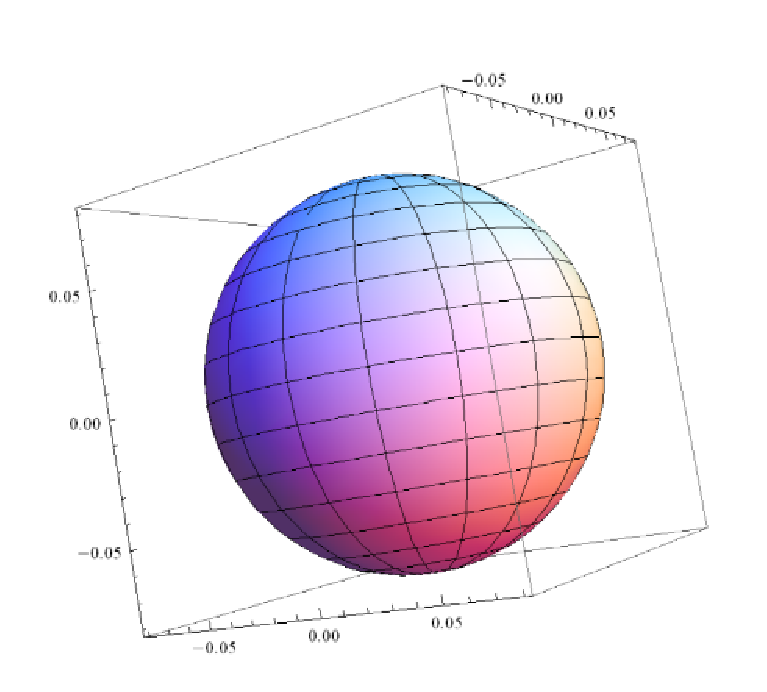
\includegraphics[width=5.722cm,height=4.842cm]{chervinskaya-1.eps}
  &
%  [Warning: Image ignored] % Unhandled or unsupported graphics:
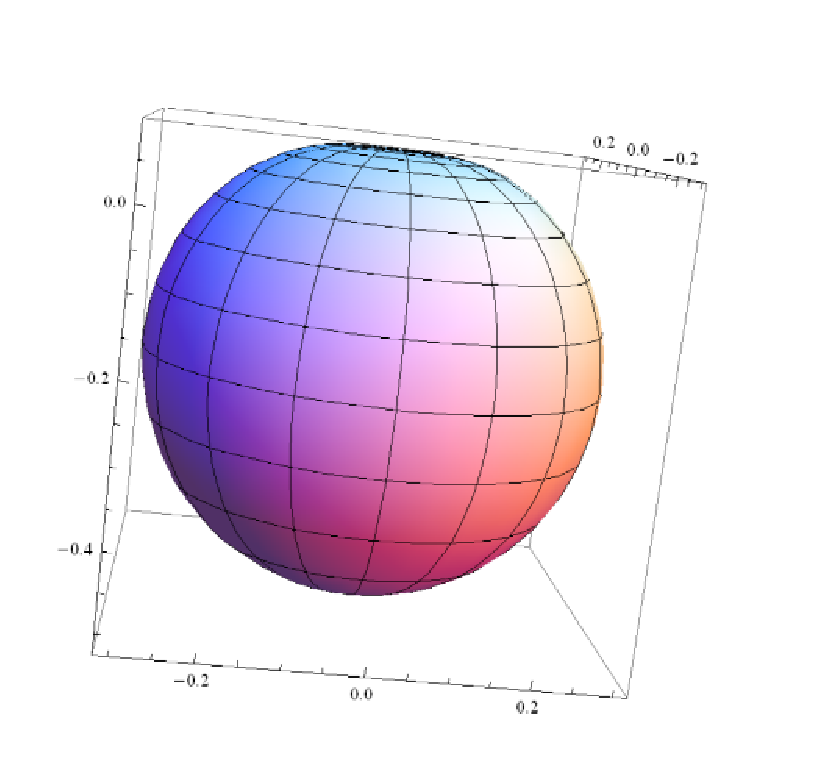
\includegraphics[width=5.106cm,height=4.748cm]{chervinskaya-2.eps}
 \\\hline
l = 1

m = 0 &
%  [Warning: Image ignored] % Unhandled or unsupported graphics:
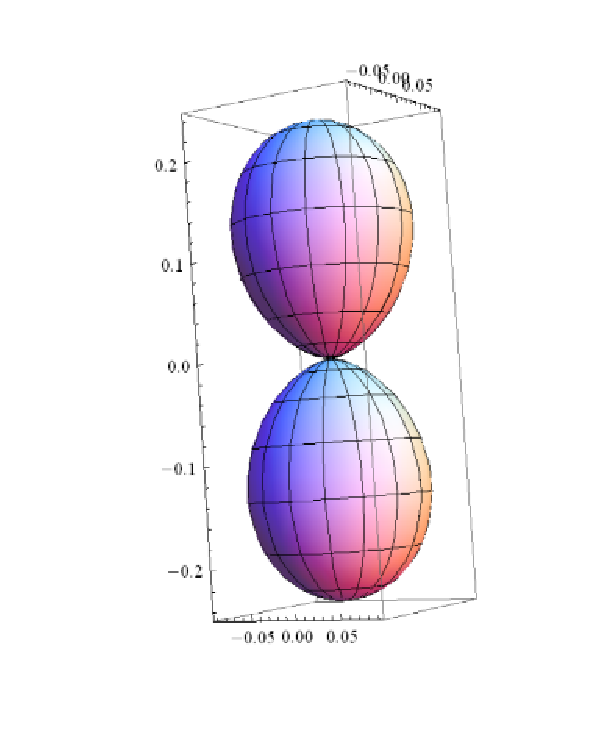
\includegraphics[width=4.948cm,height=5.9cm]{chervinskaya-3.eps}
  &
%  [Warning: Image ignored] % Unhandled or unsupported graphics:
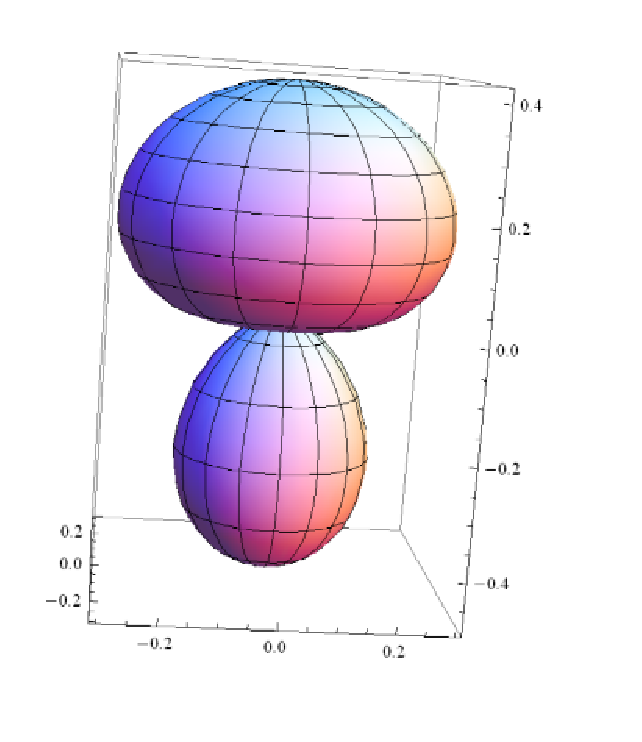
\includegraphics[width=5.027cm,height=5.457cm]{chervinskaya-4.eps}
 \\\hline
l = 2

m = 0 &
%  [Warning: Image ignored] % Unhandled or unsupported graphics:
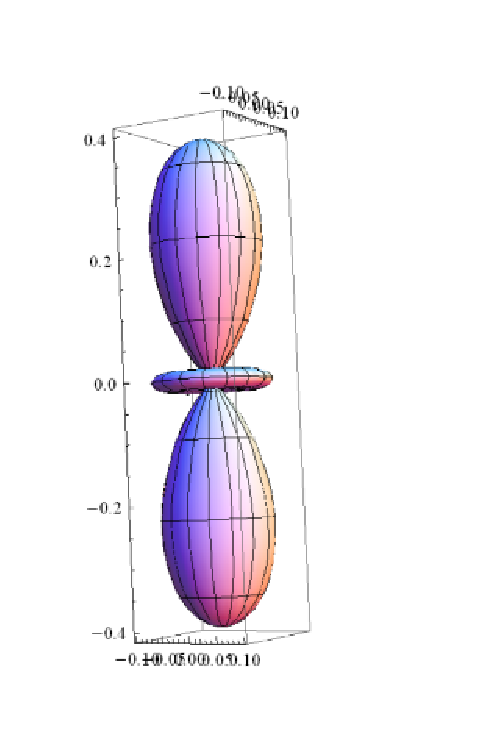
\includegraphics[width=5.292cm,height=8.44cm]{chervinskaya-5.eps}
  &
%  [Warning: Image ignored] % Unhandled or unsupported graphics:
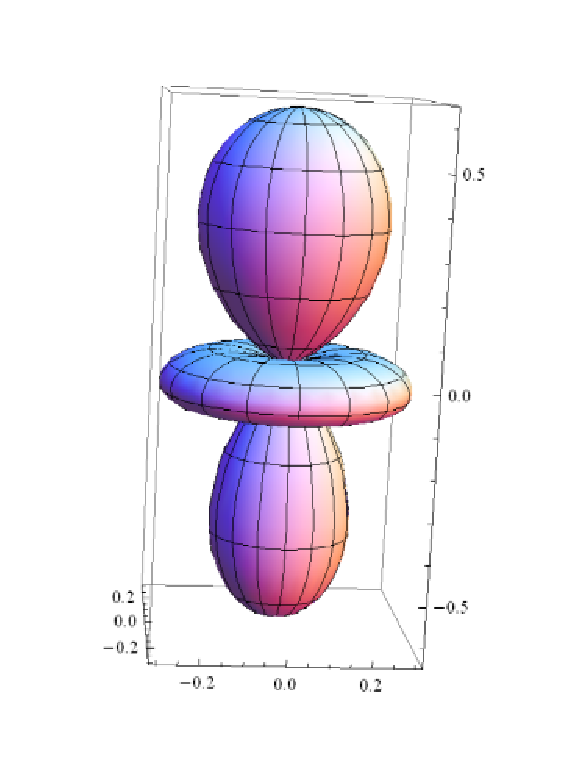
\includegraphics[width=5.136cm,height=7.646cm]{chervinskaya-6.eps}
 \\\hline
l = 1

m = 1 &
%  [Warning: Image ignored] % Unhandled or unsupported graphics:
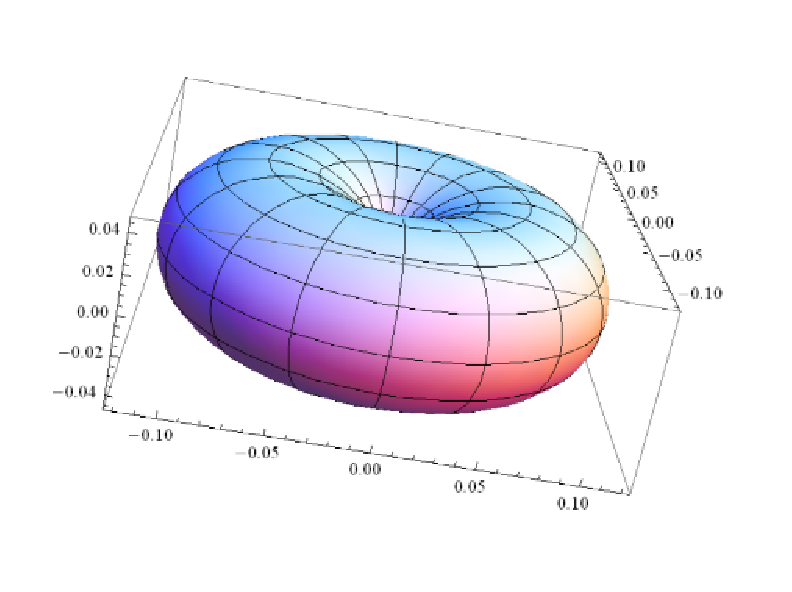
\includegraphics[width=5.72cm,height=3.731cm]{chervinskaya-7.eps}
  &
%  [Warning: Image ignored] % Unhandled or unsupported graphics:
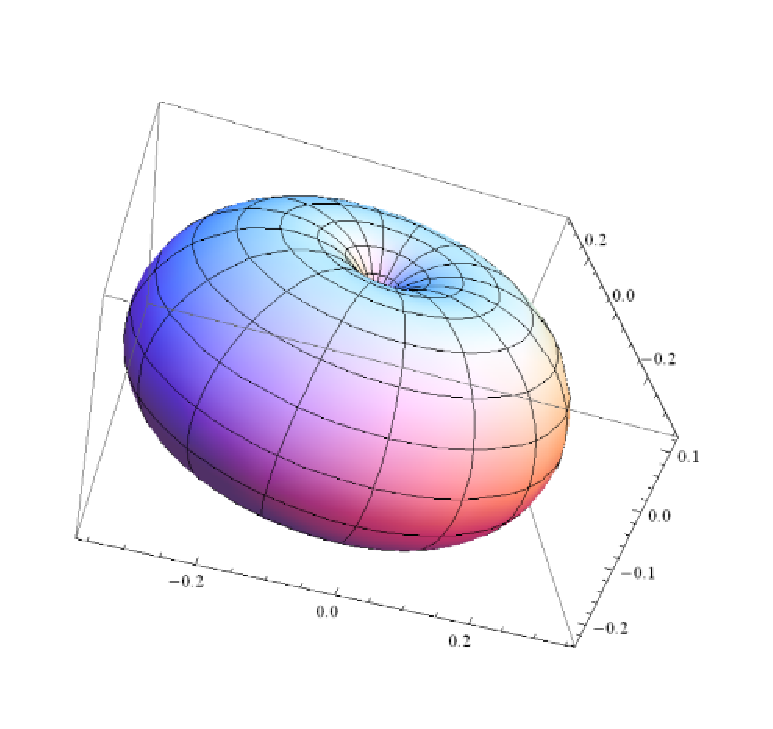
\includegraphics[width=5.099cm,height=4.26cm]{chervinskaya-8.eps}
 \\\hline
l = 1

m = 2 &
%  [Warning: Image ignored] % Unhandled or unsupported graphics:
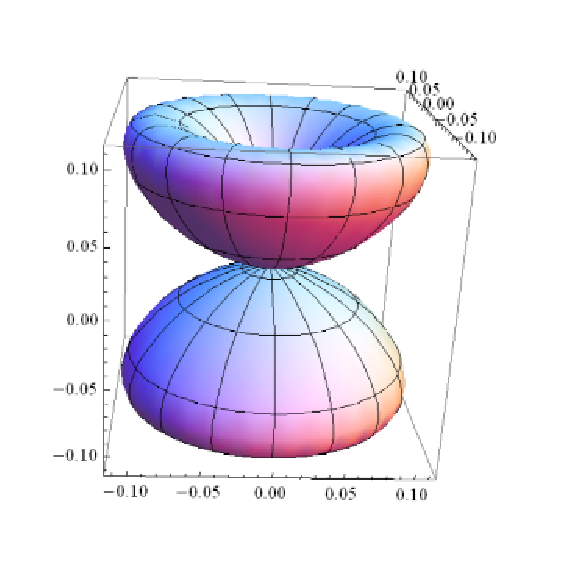
\includegraphics[width=5.292cm,height=5.078cm]{chervinskaya-9.eps}
  &
%  [Warning: Image ignored] % Unhandled or unsupported graphics:
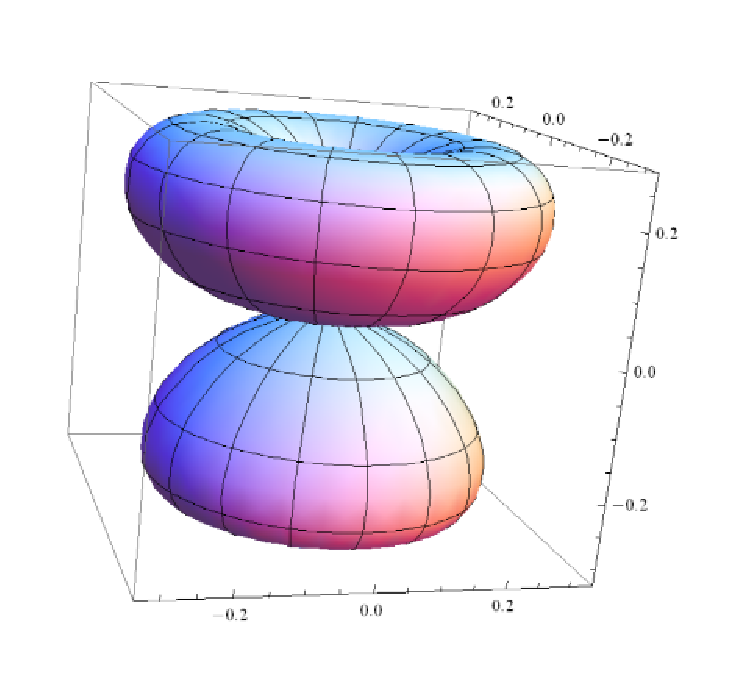
\includegraphics[width=5.98cm,height=5.017cm]{chervinskaya-10.eps}
 \\\hline
l = 2

m = 2 &
%  [Warning: Image ignored] % Unhandled or unsupported graphics:
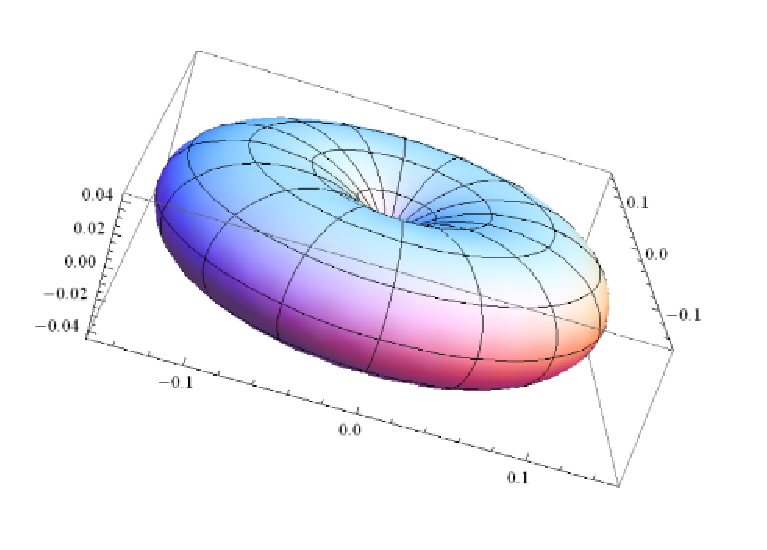
\includegraphics[width=7.541cm,height=4.916cm]{chervinskaya-11.eps}
  &
%  [Warning: Image ignored] % Unhandled or unsupported graphics:
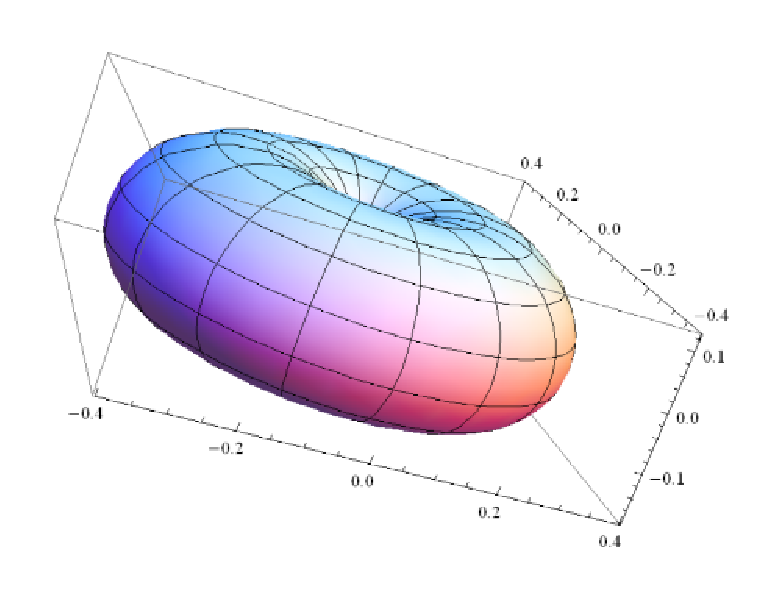
\includegraphics[width=6.773cm,height=5.48cm]{chervinskaya-12.eps}
 \\\hline
\end{tabular}







\subsubsection{Радиальная часть}
Т.к. уравнение на радиальную часть как в кулоновском, как и в кулон-дипольном случае можно свести к уравнению на фукцию Уитеккера, рассмотрим некоторые свойства этих функций, которые в дальнейшем будут нам полезны.

\paragraph{Свойства M{}- и
W{}- функций
Уитеккера[9]}
а) Уравнение на функции

\begin{equation*}
\frac{d^2W}{\mathit{dz}^2}+\left(\frac{-1} 4+\frac{\kappa } z+\frac{\frac 1 4-\mu ^2}{z^2}\right)W=0
\end{equation*}
б)  $z\rightarrow 0$

\begin{equation*}
M_{\kappa ,\mu }=z^{\mu +\frac 1 2}
\end{equation*}
В случае, если  $\frac 1 2-\kappa \pm \mu =-n$

\begin{equation*}
W_{\frac 1 2-\kappa \pm \mu ,\mu }=\left(-1\right)^n(1\pm 2\mu )_nz^{\frac 1 2\pm \mu }
\end{equation*}
Иначе

\begin{equation*}
W_{\kappa ,\mu }=\frac{\text{\textcyrillic{Г}}(2\mu )}{\text{\textcyrillic{Г}}\left(\frac 1 2+\mu -\kappa
\right)}z^{\frac 1 2-\mu }
\end{equation*}
в)  $z\rightarrow {\infty}$

\begin{equation*}
W_{\kappa ,\mu }\ e^{\frac{-1} 2z}z^k
\end{equation*}
В случае, если  $\mu -\kappa {\neq}-n-\frac 1 2$

\begin{equation*}
M_{\kappa ,\mu }(z){\sim}\frac{\Gamma (1+2\mu )e^{\frac 1 2z}z^{-\kappa }}{\Gamma (\frac 1 2+\mu -\kappa )}
\end{equation*}
\paragraph{Теоретический вывод радиальной
функции}
Рассмотрим радиальное уравнение.

\begin{equation*}
\frac 1{r^2}\frac d{\mathit{dr}}\left(r^2\frac{dR}{\mathit{dr}}\right)R+\left(\frac 2 r+2E-\frac{\lambda
}{r^2}\right)R=0(2.2.2.1)
\end{equation*}
Легко можно видеть, что по виду оно абсолютно аналогично соответствующему кулоновскому уравнению, с
заменой  $\lambda =l(l+1)$.  $\lambda $ --
собственное значение уравнения на угловую часть. Соответственно, решения будут такие же по виду.

\begin{equation*}
R=\frac 1 r\text{\textcyrillic{М}}_{\nu ,\rho }\left(r\sqrt{-8E}\right)=\frac 1
r\text{\textcyrillic{М}}_{\nu ,\rho }\left(\frac{2r}{\nu }\right)(2.2.2.2)
\end{equation*}
\begin{equation*}
E=\frac{-1}{2\nu ^2}(2.2.2.3)
\end{equation*}
\begin{equation*}
\rho _{\mathit{lm}}=\left(\lambda _{\mathit{lm}}+\frac 1 4\right)^{1/2}(2.2.2.3)
\end{equation*}
Введем понятие  $\widetilde l=\rho -\frac
1 2$ -- квазиугловой
момент.

Приведем таблицу
значений  $\widetilde l$ в
зависимости от значений дипольного момента


\begin{tabular}{|m{2.158cm}|m{2.292cm}|m{2.109cm}|m{2.112cm}|m{2.382cm}|m{2.111cm}|m{2.162cm}|}
\hline
\centering \textit{d} &
\multicolumn{3}{m{6.913cm}|}{\centering \textit{m = 0}} &
\multicolumn{2}{m{4.6930003cm}|}{\centering \textit{m = 1}} &
\textit{m = 2}\\\hline
 &
\centering \textit{l = 0} &
\centering \textit{l = 1} &
\centering \textit{l = 2} &
\centering \textit{l = 1} &
\centering \textit{l = 2} &
\centering\arraybslash \textit{l = 2}\\\hline
\raggedleft 0,2 &
\raggedleft {-0,02715} &
\raggedleft 1,00524 &
\raggedleft 2,00076 &
\raggedleft 0,997334 &
\raggedleft 2,00038 &
\raggedleft\arraybslash 1,99924\\\hline
\raggedleft 0,4 &
\raggedleft {-0,11636} &
\raggedleft 1,01989 &
\raggedleft 2,00306 &
\raggedleft 0,989341 &
\raggedleft 2,0015 &
\raggedleft\arraybslash 1,99695\\\hline
\raggedleft 0,6 &
\raggedleft {-0,33328} &
\raggedleft 1,04134 &
\raggedleft 2,00694 &
\raggedleft 0,976038 &
\raggedleft 2,00329 &
\raggedleft\arraybslash 1,99315\\\hline
\raggedleft 0,8 &
{-} &
\raggedleft 1,06655 &
\raggedleft 2,01244 &
\raggedleft 0,957442 &
\raggedleft 2,00567 &
\raggedleft\arraybslash 1,98783\\\hline
\raggedleft 1,0 &
{-} &
\raggedleft 1,09285 &
\raggedleft 2,01961 &
\raggedleft 0,933563 &
\raggedleft 2,00851 &
\raggedleft\arraybslash 1,98101\\\hline
\raggedleft 1,2 &
{-} &
\raggedleft 1,11824 &
\raggedleft 2,02852 &
\raggedleft 0,904393 &
\raggedleft 2,01168 &
\raggedleft\arraybslash 1,97268\\\hline
\raggedleft 1,4 &
{-} &
\raggedleft 1,1413 &
\raggedleft 2,03918 &
\raggedleft 0,869881 &
\raggedleft 2,01501 &
\raggedleft\arraybslash 1,96287\\\hline
\raggedleft 1,6 &
{-} &
\raggedleft 1,16111 &
\raggedleft 2,05158 &
\raggedleft 0,829924 &
\raggedleft 2,01835 &
\raggedleft\arraybslash 1,95158\\\hline
\raggedleft 1,8 &
{-} &
\raggedleft 1,17709 &
\raggedleft 2,06566 &
\raggedleft 0,784337 &
\raggedleft 2,02156 &
\raggedleft\arraybslash 1,93883\\\hline
\raggedleft 2,0 &
{-} &
\raggedleft 1,1889 &
\raggedleft 2,08132 &
\raggedleft 0,732823 &
\raggedleft 2,02448 &
\raggedleft\arraybslash 1,92462\\\hline
\end{tabular}

{\centering
Таблица 1.
\par}

Для того, чтобы выполнялись граничные условия
при  $r\rightarrow {\infty}$, необходимо,
чтобы между  $\rho $ и  $\nu $
выполнялось соотношение (см. свойство (в) п. 1.2.2.1).

\begin{equation*}
\nu =n_r+\rho +\frac 1 2(2.2.2.4)
\end{equation*}
Учитывая, что  $n=n_r+l+1$,  $\nu =n+\widetilde
l-l$

Для квантового дефекта тогда получим выражение
$\delta =l+\frac 1 2-\rho $

При использовании исключительно теоретических построений возникает следующая проблема: рассчитанные квантовые дефекты включают в себя только дипольную часть и не учитывают короткодействующую часть потенциала.

\begin{equation*}
\delta _{\mathit{calc}}{\neq}\delta _{\mathit{obs}}\rightarrow E_{\mathit{calc}}{\neq}E_{\mathit{obs}}
\end{equation*}
\paragraph{Модельный потенциал
Саймонса }

Эмпирически наблюдаемый квантовый дефект можно учесть, рассматривая модельный потенциал
следующего вида[10]:

\begin{equation*}
V\left(r\right)=\frac{\lambda \left(\lambda +1\right)-\widetilde l(\widetilde l+1)}{2r^2}-\frac 1 r(2.2.3.1)
\end{equation*}
 $\lambda $\textit{ - }параметр,
определяемый эмпирически.

Вводя замену  $R(r)=\frac{\mu (r)} r$,
получаем
уравнение на  $\mu (r)$

\begin{equation*}
\frac{-1} 2\frac{d^2\mu }{\mathit{dr}^2}+\left[\frac{\lambda (\lambda +1)}{2r^2}-\frac 1 r\right]\mu =E\mu (2.2.3.2)
\end{equation*}
Уравнение имеет следующее решение

\begin{equation*}
\mu \left(r\right)=\text{\textcyrillic{М}}_{\frac 1{\sqrt{-2E}},\lambda +\frac 1
2}\left(r\sqrt{-8E}\right)(2.2.3.3)
\end{equation*}
Энергия в этом выражении -- величина, определяемая экспериментально.

Можно воспользоваться известной формулой

\begin{equation*}
E=\frac{-1}{2(n-\delta )^2}
\end{equation*}
Тогда чтобы обеспечить
сходимость  $\text{\textcyrillic{М}}$ --
функции Уитеккера на бесконечности,

\begin{equation*}
\lambda =l-\delta +K(2.2.3.4)
\end{equation*}
 $K$\textit{ -- }целое число

Обсудим более подробно проблему выбора K.

Т.к. при малых \textit{r}
центростремительный
член  $\frac{l(l+1)}{2r^2}$
преобладает в
\textit{V}\textit{(}\textit{r}\textit{)},
Саймонс в оригинальной
статье [10, стр. 646]
предлагает
определить \textit{K}
таким образом,
чтобы  $| \lambda -l| $ был
минимальным.

Тогда  $k=\mathit{Round}(\delta )$

 $\mathit{Round}\left(\delta \right)$\textit{ -- }ближайшее
к  $\delta $ целое число.

В статье 1995 года [11, стр.
311] Мартин, довольно
подробно обсуждая
проблему выбора  $k$,
указывает на то, что количество узлов радиальной
функции равно  $n-l-k-1$.

С математической точки зрения допустимы следующие
значения \textit{k}

\begin{equation*}
\delta -l-\frac 3 2<k{\leq}n-l-1
\end{equation*}
В качестве возможного выбора
Мартин приводит  $k=0$. В
этом случае количество узлов в волновой функции такое же, как у соответствующей волновой функции атома водорода.

В собственной работе Мартин
использует  $c=2-l$ для  $l=0,1,2$.
В этом случае радиальная волновая функция
при  $n=l$ не имеет узлов.

В статье 2002 года [12, стр.75]
Алчеев, также обсуждая проблему выбора k, использует для него следующее выражение.

\begin{equation*}
\lambda =n-\delta -k-1
\end{equation*}
Алчеев определяет  $k$
таким образом:

\begin{equation*}
k=n-n_{\mathit{cl}}(2.2.3.5)
\end{equation*}
 $n_{\mathit{cl}}$\textit{ -- }количество
заполненных электронных оболочек.

Можно сделать вывод, что рассмотренные авторы определяют параметр k существенно по-разному, хотя результат расчета радиального матричного элемента может сильно зависеть от этого параметра.

\paragraph{Метод
Бейтс-Дамгард }
В методе, предложенном в статье Бейтса-Дамгард 1949
года [13], потенциал
заменяется на

\begin{equation*}
V=\frac 1 r
\end{equation*}
При этом энергия, входящая в уравнение, не является его собственным значением, а является экспериментально измеренной величиной.

\begin{equation*}
\frac{d^2R}{\mathit{dr}^2}+\left(\frac 2 r-\frac{l(l+1)}{r^2}-E\right)R=0
\end{equation*}
 $E$ -- энергия,
измеренная экспериментальным образом

Решение должно удовлетворять граничным
условиям  $R\rightarrow 0$ при $r\rightarrow {\infty}$

Т.к.  $E$ - не собственное
значение дифференциального уравнения, решение будет расходиться
при  $r\rightarrow 0$.

Для нас наиболее подходящим будет решение

\begin{equation*}
R=W_{\nu _{\mathit{klm}},l+\frac 1 2}\left(\frac{2r}{\nu _{\mathit{klm}}}\right)(2.2.4.1)
\end{equation*}
При этом нормировочный фактор будет:

\begin{equation*}
N=\frac 1{\sqrt{\nu _{\mathit{klm}}\text{\textcyrillic{Г}}(\nu
_{\mathit{klm}}+l-1)\text{\textcyrillic{Г}}(\nu _{\mathit{klm}}-l)}}(2.2.4.2)
\end{equation*}
В наших расчетах  $l\rightarrow
\widetilde l$.

Конечный вид радиальной части будет следующим:

\begin{equation*}
R=\left(1+\frac{d\delta _{\mathit{lm}}}{d\nu _{\mathit{klm}}}\right)^{-1/2}\left(\nu
_{\mathit{klm}}\text{\textcyrillic{Г}}(\nu _{\mathit{klm}}+\widetilde l-1)\text{\textcyrillic{Г}}(\nu
_{\mathit{klm}}-\widetilde l)\right)^{-1/2}W_{\nu _{\mathit{klm}},\widetilde l+\frac 1 2}\left(\frac{2r}{\nu
_{\mathit{klm}}}\right)(2.2.4.3)
\end{equation*}
Нормировочный фактор  $\left(1+\frac{d\delta _{\mathit{lm}}}{d\nu _{\mathit{klm}}}\right)^{-1/2}$
был предложен и выведен Ситоном  в статье 1958 [14].

Рассмотрим отдельно проблему с невыполнением граничных условий (при  $r\rightarrow 0,R\rightarrow \mathit{ComplexInfinity}$)

Данную проблему можно решить путем введения эффективного радиуса, который представляет собой классическую точку поворота [15].
\begin{equation*}
 \frac{\lambda }{r^2}-\frac 2 r=\frac{-1}{\nu _{\mathit{klm}}^2}
\end{equation*}
\begin{equation*}
 \frac{r^2}{\nu _{\mathit{klm}}^2}-2r+\lambda =0
\end{equation*}
\begin{equation*}
 r_c=\left(1-\sqrt{1-\frac{\widetilde l(\widetilde l+1)}{\nu _{\mathit{klm}}^2}}\right)\nu
_{\mathit{klm}}^2(2.2.4.4)
\end{equation*}



\textbf{Сводная таблица (для радиальной части)}

\begin{equation*}
R=W_{\nu ,\rho }\left(\frac{2r}{\nu }\right)
\end{equation*}


\begin{tabular}{|m{2.723cm}|m{2.61cm}|m{3.931cm}|m{3.155cm}|m{3.222cm}|}
\hline
~
 &
 $\nu $ &
 $\rho $ &
\textbf{Особенности} &
\centering\arraybslash \textbf{Нижний
предел
интегрирования}\\\hline
\textbf{Модельный
потенциал
Саймонса} &
 $\nu _{\mathit{obs}}$ &
 $l-n+\nu _{\mathit{obs}}+K+\frac 1 2$ &
Нужно подбирать
k &
\textbf{0}\\\hline
\textbf{Метод
Бейтса-Дамгаард} &
 $\nu _{\mathit{obs}}$ &
 $\widetilde l_{\mathit{lm}}+\frac 1 2$ &
Расходится в 0 &
 $\left(1-\sqrt{1-\frac{\widetilde l(\widetilde l+1)}{\nu _{\mathit{klm}}^2}}\right)\nu _{\mathit{klm}}^2$\\\hline
\end{tabular}

{\centering
\textbf{Таблица 2.}
\par}




\textbf{Сравнение
графиков (нормированных) радиальных функций, построенных различными
способами}

\textbf{(}\textbf{NaHe}\textbf{, }\textbf{n}\textbf{ = 3,
}\textbf{l}\textbf{ = 1, }\textbf{m}\textbf{ = 0)}

%  [Warning: Image ignored] % Unhandled or unsupported graphics:
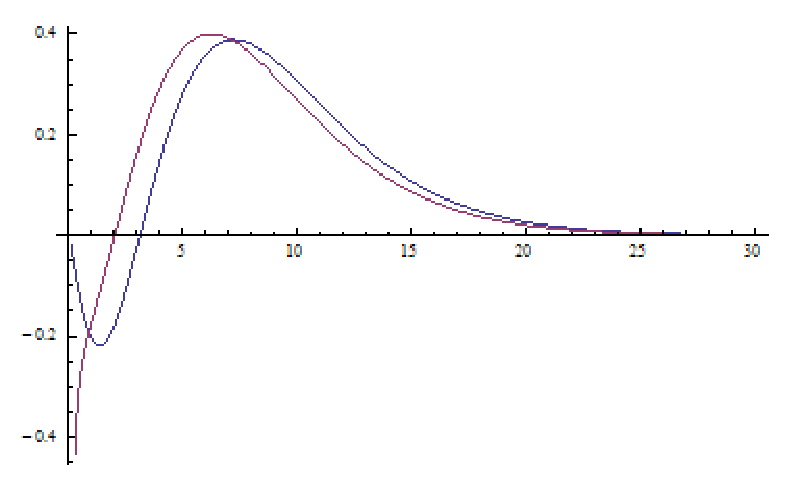
\includegraphics[width=9.537cm,height=5.655cm]{chervinskaya-14.eps}



%TODO: разобраться, что за дрянь
\begin{tabular}{m{3.741cm}m{12.927cm}}
[Warning: Draw object ignored] &
Модельный потенциал
Саймонса\\
{}[Warning: Draw object ignored] &
Метод
Бейтса-Дамгард\\
\end{tabular}




\textbf{(}\textbf{NaHe}\textbf{, }\textbf{n}\textbf{ = 3,
}\textbf{l}\textbf{ = }\textbf{0}\textbf{,
}\textbf{m}\textbf{ = 0)}

%  [Warning: Image ignored] % Unhandled or unsupported graphics:
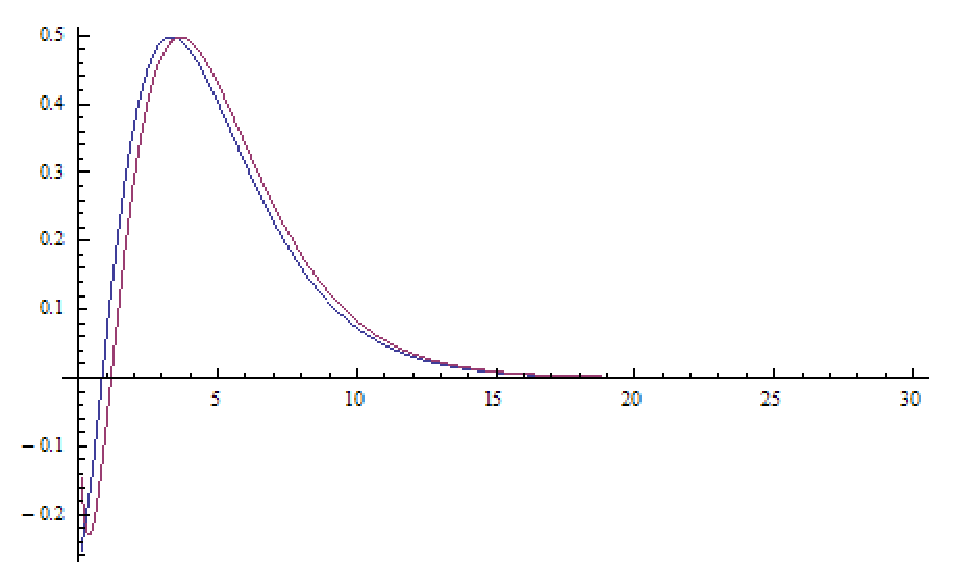
\includegraphics[width=11.592cm,height=6.904cm]{chervinskaya-15.eps}



\begin{tabular}{m{3.741cm}m{12.927cm}}
[Warning: Draw object ignored] &
Модельный потенциал
Саймонса\\
{}[Warning: Draw object ignored] &
Метод
Бейтса-Дамгард\\
\end{tabular}

\clearpage\subsection{Вычисление сил
осцилляторов}
\subsubsection{Понятие
силы осциллятора. Переходы между состояниями дискретного
спектра.}
Для перехода
из состояния $a$
в состояние $b$
сила осциллятора
определяется как [16]

\begin{equation*}
	f_{ab}=
	\frac{2}{3}\left( E_b-E_a \right) \left| \left< \psi_b |\textbf{d}| \psi_a \right> \right|^2
\end{equation*}
\begin{equation*}
{\textbf{d}} = \sum _n\ \textbf{r}_n
\end{equation*}
Суммирование производится по всем электронам.

Вероятность
перехода $a$ в
состояние $b$,
для которых  $E_b>E_a$,
определяется через силу осциллятора таким образом:

\begin{equation*}
\text{\textcyrillic{Г}}_R\left(b\rightarrow a\right)=\frac{2\alpha ^3}{\tau
_0}\left(E_b-E_a\right)^2f_{\mathit{ba}}
\end{equation*}
 $\alpha {\approx}\frac 1{137}$\textit{ }{}- постоянная
тонкой структуры

 $\tau _0$\textit{ -- }атомная
единица времени

Так как волновая функция разделяется на радиальную и угловую части, мы можем сосчитать отдельно угловой и радиальный матричный элементы

Для нашей системы сила осциллятора будет выглядеть таким образом:

\begin{equation*}
f_{ab}=\frac 2 3 \left(E_b-E_a\right) \left| \left< n_1l_1m_1\left|r\right|n_2l_2m_2 \right> \right|^2 Q\left(\widetilde l_1m_1\rightarrow \widetilde l_2m_2\right) (3.1.2)
\end{equation*}
\subsubsection{Расчет
угловой части дипольного матричного
элемента}
Посчитаем
дипольный матричный элемент  $Q\left(\widetilde l_1m_1\rightarrow \widetilde l_2m_2\right)$.

Угловая часть нашей волновой функции есть диполь-сферическая функция. Угловые части радиус-вектора выражается через сферические гармоники  $Y_{1m}$.
Сосчитаем матричный элемент следующего вида:
\begin{multline*}
\left<\widetilde Y_{l_1 m_1}|Y_{1m}|\widetilde Y_{l_2 m_2} \right> =\sum_{l'_1=|m_1 |}^{\infty}\sum_{l'_2=|m_2|}^{\infty}a_{l_1 m_1}^{l'_1} a_{l_2 m_2}^{l'_2} \int Y_{l'_1 m_1} Y_{1m} Y_{l'_2 m_2}^* d\Omega=
\\
=\sum_{l'_1=|m_1|}^{\infty} \sum_{l'_2=|m_2 |}^{\infty} a_{l_1 m_1}^{l'_1} a_{l_2 m_2}^{l'_2} \int Y_{l'_1 m_1} Y_{1m} Y_{l'_2 m_2}^* d\Omega   (3.2.1)
\end{multline*}
Отдельно вычислим входящий в данное выражение интеграл.
\begin{equation*}
	\int Y_{l'_1m_1}Y_{1m}Y_{l'_2m_2}^{\ast }\mathit{d\Omega }=
	\sqrt{
		\frac{3(2l^{'}_{1}+1)}{4\pi (2l{'}_2 +1)}
	}
	C_{l{'}_{1010}}^{l{'}_{20}}C_{l{'}_1 m_11 m}^{l{'}_2m_2}
	(3.2.2)
\end{equation*}
Теперь, подставив (3.2.2) в (3.2.1) и воспользовавшись известными выражениями угловой части радиус-вектора через сферические гармоники, можем вычислить угловую часть дипольного матричного элемента.
\begin{multline*}
Q_x\left(l_1m_1\rightarrow l_2m_2\right)=\sqrt{\frac{2\pi } 3} \left< \widetilde Y_{l_1m_1}|Y_{1-1}-Y_{11}|\widetilde Y_{l_2m_2} \right> =
\\
= \frac{\delta_{m_1-1 m_2}}{\sqrt{2}}\sum_{l'_1=|m_1|}^{\infty} \sum_{l'_2=|m_2|}^{\infty}\sqrt{\frac{2l'_1+1}{2l'_2+1}}a_{l_1 m_1}^{l'_1 } a_{l_2 m_2}^{l'_2} C_{l'_1 010}^{l'_2 0} C_{l'_1 m_1 1-1}^{l'_2 m_2 }-
\\
\frac{\delta_{m_1+1 m_2}}{\sqrt{2}}\sum_{l'_1=|m_1|}^{\infty} \sum_{l'_2=|m_2|}^{\infty}\sqrt{\frac{2l'_1+1}{2l'_2+1}}a_{l_1 m_1}^{l'_1 } a_{l_2 m_2}^{l'_2} C_{l'_1 010}^{l'_2 0} C_{l'_1 m_1 1-1}^{l'_2 m_2 }
\end{multline*}
\begin{multline*}
Q_y\left(l_1m_1\rightarrow l_2m_2\right)=i\sqrt{\frac{2\pi } 3} \left< \widetilde Y_{l_1m_1}|Y_{1-1}+Y_{11}|\widetilde Y_{l_2m_2} \right> =
\\
= i\frac{\delta_{m_1-1 m_2}}{\sqrt{2}}\sum_{l'_1=|m_1|}^{\infty} \sum_{l'_2=|m_2|}^{\infty}\sqrt{\frac{2l'_1+1}{2l'_2+1}}a_{l_1 m_1}^{l'_1 } a_{l_2 m_2}^{l'_2} C_{l'_1 010}^{l'_2 0} C_{l'_1 m_1 1-1}^{l'_2 m_2 }+
\\
i\frac{\delta_{m_1+1 m_2}}{\sqrt{2}}\sum_{l'_1=|m_1|}^{\infty} \sum_{l'_2=|m_2|}^{\infty}\sqrt{\frac{2l'_1+1}{2l'_2+1}}a_{l_1 m_1}^{l'_1 } a_{l_2 m_2}^{l'_2} C_{l'_1 010}^{l'_2 0} C_{l'_1 m_1 1-1}^{l'_2 m_2 }
\end{multline*}
\begin{multline*}
Q_z\left(l_1m_1\rightarrow l_2m_2\right)=\sqrt{\frac{4\pi } 3} \left< \widetilde Y_{l_1m_1}|Y_{10}|\widetilde Y_{l_2m_2} \right> =
\\
= \delta_{m_1-1 m_2}\sum_{l'_1=|m_1|}^{\infty} \sum_{l'_2=|m_2|}^{\infty}\sqrt{\frac{2l'_1+1}{2l'_2+1}}a_{l_1 m_1}^{l'_1 } a_{l_2 m_2}^{l'_2} C_{l'_1 010}^{l'_2 0} C_{l'_1 m_1 1-1}^{l'_2 m_2 }
\end{multline*}
Теперь вычислим квадрат модуля угловой части дипольного матричного элемента, получив такое конечное выражение:
\begin{multline*}
	Q\left(l_1m_1\rightarrow l_2m_2\right)^2=
Q_x\left(l_1m_1\rightarrow l_2m_2\right)^2+Q_y\left(l_1m_1\rightarrow l_2m_2\right)^2+Q_z\left(l_1m_1\rightarrow l_2m_2\right)^2 =
\\
= \left(2-\delta _{0m_0}\right)\left(\sum _{l'_1=| m_1|
	?}^{\infty}\sum _{l'_2=| m_2|
	?}^{\infty} \sqrt{\frac{2l^{'}_1+1}{2l{'}_2+1}}a_{l_1m_1}^{l{'}_1}a_{l_2m_2}^{l{'}_2}C_{l{'}_1010}^{l{'}_20}C_{l{'}_1 m_11 m_2-m_1}^{l{'}_2m_2}\right)^2(3.2.5)
\end{multline*}
Множитель  $2-\delta _{0m_0}$ соответствует необходимости учитывать двукратное вырождение системы при  $m_0{\neq}0$.{[12]}

\subsection{Потенциал
реальных двухатомных систем. Двухцентровый
потенциал.}
{\centering [Warning: Draw object ignored]\par}
Ридберговское состояние двухатомной системы можно представить, как ион с двумя зарядовыми центрами и удаленный от него электрон.

Рассмотрим, как выглядит потенциал системы из двух зарядов, удаленных друг от друга на
расстояние $l$, с суммарным зарядом $Z=1$. Система
изображена на рис.1.

\begin{equation*}
\varphi =\frac q{\sqrt{r^2+(l-b)^2+2(l-b)x}}+\frac{1-q}{\sqrt{r^2+b^2-2\mathit{bx}}}
\end{equation*}
Потенциал такой системы можно представить в виде суммы кулоновского и дипольного потенциала. Рассчитаем дипольный и квадрупольный моменты такой системы.

\begin{equation*}
d=\left(1-q\right)b+q\left(b-l\right)=b-\mathit{ql}
\end{equation*}
\begin{equation*}
Q_{\mathit{xx}}=2b^2\left(1-q\right)+2q\left(b-l\right)^2=2\left(b^2-2q\mathit{bl}+ql^2\right)
\end{equation*}
Мы решали задачу о ридберговском электроне в дипольном приближении, поэтому, пользуясь неинвариантностью высших мультипольных моментов системы в зависимости от выбора системы отсчета, выберем систему отсчета таким образом, чтобы квадрупольный член был равен 0.

\begin{equation*}
b^2-2\mathit{blq}+ql^2=0
\end{equation*}
Обратим внимание на то, что если оба заряда системы положительны, выбрать таким образом систему отсчета не удается.

\begin{equation*}
b=\mathit{ql}\pm l\sqrt{q\left(q-1\right)}
\end{equation*}
Рассчитав, где должна находиться точка отчета, определим дипольный момент.

\begin{equation*}
d=l\sqrt{q\left(q-1\right)}
\end{equation*}
Рассмотрим такую систему отсчета, центр которой находится посередине двух зарядов. Рассмотрим мультипольные моменты относительно такой системы отсчета.

\begin{equation*}
d_0=l\left(\frac 1 2-q\right)
\end{equation*}
\begin{equation*}
Q_0=\frac l 4^2
\end{equation*}
Рассмотрим комбинацию  $d_0^2-Q_0$.

\begin{equation*}
d_0^2-Q_0=l^2\left(\frac 1 4-q+q^2\right)-\frac l 4^2=l^2\left(q^2-q\right)=d^2
\end{equation*}
 $d=\sqrt{d_0^2-Q_0}$ -- эффективный дипольный момент, инвариантный относительно выбора системы отсчета. Обратим внимание на то, что такая комбинация существует только в том
случае, если  $d_0^2>Q_0$.

На рис. 2 (а,б) приведено сравнение двухцентрового потенциала с дипольным, построенным таким образом.


\begin{tabular}{m{8.216001cm}m{8.265cm}}
{\centering   %[Warning: Image ignored] % Unhandled or unsupported graphics:
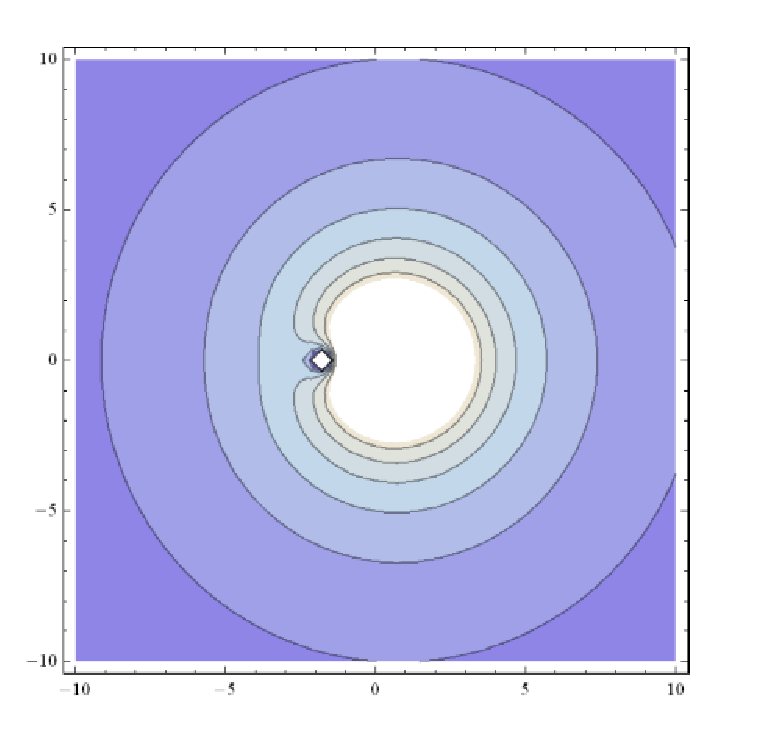
\includegraphics[width=7.265cm,height=7.165cm]{chervinskaya-16.eps}
 \par}
\centering а) Двухцентровый
потенциал &
{\centering   %[Warning: Image ignored] % Unhandled or unsupported graphics:
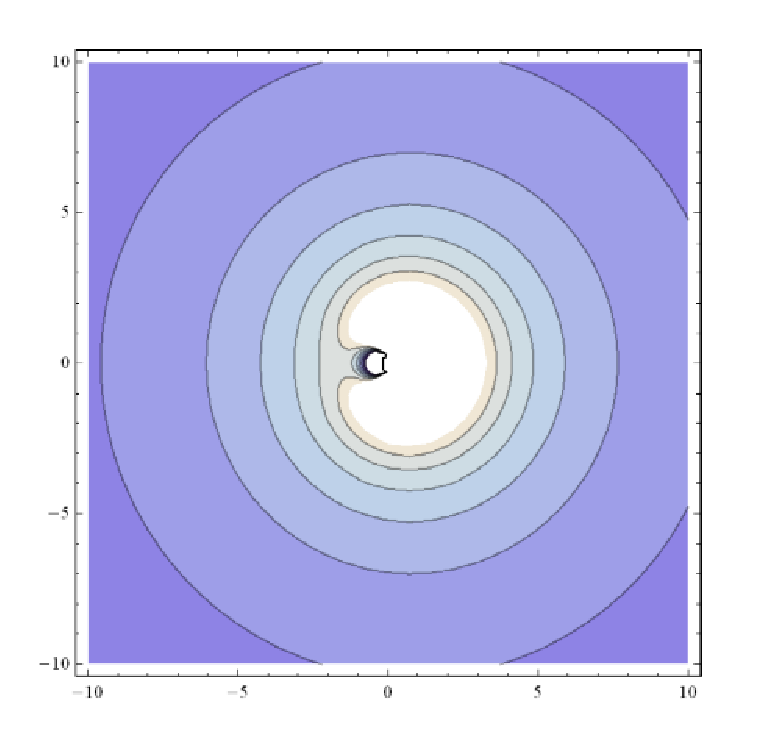
\includegraphics[width=7.303cm,height=7.2cm]{chervinskaya-17.eps}
 \par}
\centering\arraybslash б)
Двухцентровый
потенциал\\
\multicolumn{2}{m{16.681cm}}{\centering Рис.2}\\
\end{tabular}



\clearpage\section{Расчет
сил осцилляторов}
\subsection{Расчеты ab
initio}

В работе мы планируем исследовать молекулы $NaHe$, $CaF$, $NeH$.
Часть параметров, которые нам необходимы для использования метода $QDT$, мы можем узнать, произведя компьютерный расчет $ab initio$ основного состояния ионов соответствующих молекул.
Такими параметрами являются вращательные константы, дипольные и квадрупольные моменты.  Будем использовать для этого программы Gaussian 09W и GaussView 5.0.

Пример кода программы для расчета оптимальной конфигурации иона
NaHe+.

\#p opt MP4/aug-cc-pV5Z

NaHe

1 1

Na \ \ \ \ \ \ \ \ \ \ \ \

He 1 R

R 2.31

Видно, что производится оптимизация межъядерного расстояния в ионе NaHe+ методом Мольера--Плиссе 4-го порядка (MP4) с используемым базисом aug-cc-pV5Z.
Для молекулы CaF были использованы экспериментальные результаты, полученные Jungen в 2001 году.

Приведем для каждого иона сводную таблицу полученных результатов.


\begin{tabular}{|m{1.495cm}|m{2.3539999cm}|m{2.781cm}|m{2.76cm}|m{2.899cm}|m{2.9359999cm}|}
\hline
\textbf{Метод расчета} &
\textbf{Базис} &
\textbf{B (а.е.)} &
\textbf{Дипольный
момент, a.u.} &
\textbf{Квадрупольный
момент, a.u.} &
\textbf{Эффективный
дипольный момент,
a.u.}\\\hline
\centering MP2 &
6-31++g &
\raggedleft  $5,14\ast 10^{-7}$ &
\raggedleft 0,65 &
\raggedleft 0,20 &
\raggedleft\arraybslash 0,47\\\hline
\centering MP4 &
6-31++g &
\raggedleft  $5,11\ast 10^{-7}$ &
\raggedleft 0,75 &
\raggedleft 0,24 &
\raggedleft\arraybslash 0,57\\\hline
 &
aug-cc-pVTZ &
\raggedleft  $6,13\ast 10^{-7}$ &
\raggedleft \textit{0,60} &
\raggedleft \textit{0,30} &
\raggedleft\arraybslash 0,24\\\hhline{~-----}
 &
aug-cc-pV5Z &
\raggedleft  $6,13\ast 10^{-7}$ &
\raggedleft \textit{0,60} &
\raggedleft \textit{0,30} &
\raggedleft\arraybslash 0,24\\\hline
\centering HF &
6-31++g &
\raggedleft  $5,11\ast 10^{-7}$ &
\raggedleft \textit{0,75} &
\raggedleft \textit{0,24} &
\raggedleft\arraybslash 0,57\\\hline
 &
aug-cc-pVTZ &
\raggedleft  $6,14\ast 10^{-7}$ &
\raggedleft 0,64 &
\raggedleft 0,32 &
\raggedleft\arraybslash 0,30\\\hline
\centering CCSD(T) &
6-31++g &
\raggedleft  $5,11\ast 10^{-7}$ &
\raggedleft 0,75 &
\raggedleft 0,24 &
\raggedleft\arraybslash 0,57\\\hline
 &
aug-cc-pVTZ &
\raggedleft  $6,14\ast 10^{-7}$ &
\raggedleft 0,64 &
\raggedleft 0,32 &
\raggedleft\arraybslash 0,30\\\hhline{~-----}
\end{tabular}

{\centering
Таблица 4. Ион NaHe+
\par}



\begin{tabular}{|m{1.8989999cm}|m{2.476cm}|m{2.2979999cm}|m{2.294cm}|m{2.917cm}|m{3.2849998cm}|}
\hline
\textbf{Метод расчета} &
\textbf{Базис} &
\textbf{B (а.е.)} &
\textbf{Дипольный
момент, a.u.} &
\textbf{Квадрупольный
момент, a.u.} &
\textbf{Эффективный
дипольный момент,
a.u.}\\\hline
\centering {MP2} &
{6-31++g} &
\raggedleft  $2,14\ast 10^{-7}$ &
\raggedleft {5,00} &
\raggedleft {{}-1,28} &
\raggedleft\arraybslash {5,13}\\\hline
\centering {MP4} &
{6-31++g} &
\raggedleft  $2,14\ast 10^{-7}$ &
\raggedleft {5,02} &
\raggedleft {{}-1,29} &
\raggedleft\arraybslash {5,15}\\\hline
 &
{aug-cc-pVTZ} &
{{}-{}-} &
~
 &
~
 &
~
\\\hhline{~-----}
 &
{aug-cc-pV5Z} &
{{}-{}-} &
~
 &
~
 &
~
\\\hline
\centering {HF} &
{6-31++g} &
\raggedleft  $2,23\ast 10^{-7}$ &
\raggedleft \textit{4,91} &
\raggedleft \textit{{{}-1,26}} &
\raggedleft\arraybslash {5,04}\\\hline
 &
{aug-cc-pVTZ} &
{{}-{}-} &
~
 &
~
 &
~
\\\hline
\centering {CCSD(T)} &
{6-31++g} &
\raggedleft  $2,15\ast 10^{-7}$ &
\raggedleft {5,00} &
\raggedleft {{}-1,29} &
\raggedleft\arraybslash {5,12}\\\hline
 &
{aug-cc-pVTZ} &
{{}-{}-} &
~
 &
~
 &
~
\\\hhline{------}
\end{tabular}

{\centering
{Таблица 5. Ион
}{CaF}{+}
\par}


\begin{tabular}{|m{1.813cm}|m{2.536cm}|m{2.284cm}|m{2.245cm}|m{2.8969998cm}|m{3.405cm}|}
\hline
\textbf{Метод расчета} &
\textbf{Базис} &
\textbf{B (а.е.)} &
\textbf{Дипольный
момент, a.u.} &
\textbf{Квадрупольный
момент, a.u.} &
\textbf{Эффективный
дипольный момент,
a.u.}\\\hline
\centering {MP2} &
{6-31++g} &
\raggedleft  $1,11\ast 10^{-5}$ &
\raggedleft {1,40} &
\raggedleft {0,94} &
\raggedleft\arraybslash {1,01}\\\hline
\centering {MP4} &
{6-31++g} &
\raggedleft  $1,11\ast 10^{-5}$ &
\raggedleft {1,40} &
\raggedleft {0,94} &
\raggedleft\arraybslash {1,01}\\\hline
 &
{aug-cc-pVTZ} &
\raggedleft  $1,29\ast 10^{-5}$ &
\raggedleft \textit{1,17} &
\raggedleft {0,89} &
\raggedleft\arraybslash {0,70}\\\hhline{------}
 &
{aug-cc-pV5Z} &
{{-{}-{}-}} &
\textit{{{-{}-{}-}}} &
\textit{{{-{}-{}-}}} &
~
\\\hline
\centering {HF} &
{6-31++g} &
\raggedleft  $1,16\ast 10^{-5}$ &
\raggedleft \textit{1,35} &
\raggedleft \textit{0,90} &
\raggedleft\arraybslash {0,97}\\\hline
 &
{aug-cc-pVTZ} &
\raggedleft  $1,35\ast 10^{-5}$ &
\raggedleft {1,07} &
\raggedleft {0,77} &
\raggedleft\arraybslash {0,61}\\\hline
\centering {CCSD(T)} &
{6-31++g} &
\raggedleft  $1,11\ast 10^{-5}$ &
\raggedleft {1,39} &
\raggedleft {0,94} &
\raggedleft\arraybslash {1,00}\\\hline
 &
{aug-cc-pVTZ} &
\raggedleft  $1,29\ast 10^{-5}$ &
\raggedleft {1,10} &
\raggedleft {0,81} &
\raggedleft\arraybslash {0,64}\\\hhline{------}
\end{tabular}

{\centering
{Таблица
}{6}{. Ион
}{NeH}{+}
\par}

\subsection{Определение
применимости прямого приближения
Борна-Оппенгеймера.}
Определим, при каких условиях для исследуемых молекул выполняется
соотношение  $(1.1)$,
которое позволяет использовать прямое приближение Борна-Оппенгеймера.

\begin{equation*}
4\mathit{BJ}{\ll}\frac{\mu }{n^3}
\end{equation*}
Среди серий берем серию с минимальным квантовым дефектом. Квантовый дефект усредняем по
$n$. Для каждой молекулы оцениваем $n$, при котором соотношение перестает выполняться.


\begin{tabular}{|m{1.8cm}|m{1.3cm}|m{2.7319999cm}|m{3.726cm}|m{4.353cm}|}
\hline
\textbf{Молекула} &
\textbf{$\mu$} &
\textbf{Серия} &
\textbf{B (а.е.)} &
\textbf{n}\\\hline
{NaHe} &
\raggedleft {{}-0,089} &
{Пd} &
\raggedleft  $6,175\ast 10^{-7}$ &
\raggedleft\arraybslash {33}\\\hline
{CaF} &
\raggedleft {0,023} &
{$\Delta $f} &
\raggedleft  $2,126\ast 10^{-7}$ &
\raggedleft\arraybslash {30}\\\hline
{NeH} &
\raggedleft {{}-0,03}{9} &
{$\Sigma $d} &
\raggedleft  $1,295\ast 10^{-5}$ &
\raggedleft\arraybslash {9}\\\hline
\end{tabular}

{\centering
{Таблица }{4}
\par}

Видно, что соотношение перестает выполняться при достаточно
больших $n$.

\subsection{Значения сил осцилляторов для молекулы NaHe. Запрещенные
переходы.}
{\centering
\textbf{Зависимость
квантового
дефекта от }\textbf{n}\textbf{
для }\textbf{NaHe}
\par}

Квантовые дефекты приведены по статье Theodorakopoulus G. and Petsalakis,. D. 1993 года
[19]




{\centering
\textbf{Силы
осцилляторов (NaHe)}
\par}


\begin{tabular}{|m{4.3650002cm}|m{5.1150002cm}|m{5.464cm}|}
\hline
\textbf{Переход} &
\textbf{f }\textbf{\textsubscript{osc }}\textbf{* 1000} &
\textbf{f }\textbf{\textsubscript{osc}}\textbf{ * 1000
}\textbf{[17]}\\\hline
{$\Sigma $ (3s) $\rightarrow $ П (3p)} &
\raggedleft {55}{3} &
\raggedleft\arraybslash {561}\\
{$\Sigma $ (3s) $\rightarrow $ П (4p)} &
\raggedleft {0,5}{1} &
\raggedleft\arraybslash {6,41}\\
{$\Sigma $ (3s) $\rightarrow $ П (5p)} &
\raggedleft {1,3}{1} &
\raggedleft\arraybslash {1,33}\\
{$\Sigma $ (3s) $\rightarrow $ П (6p)} &
\raggedleft {0,16}{3} &
\raggedleft\arraybslash {0,165}\\
{$\Sigma $ (3s) $\rightarrow $ П (7p)} &
\raggedleft {0,0942} &
\raggedleft\arraybslash {0,0947}\\
{$\Sigma $ (3s) $\rightarrow $ П (8p)} &
\raggedleft {0,0208} &
\raggedleft\arraybslash {0,0215}\\
{$\Sigma $ (3s) $\rightarrow $ П (9p)} &
\raggedleft {0,01}{2} &
\raggedleft\arraybslash {0,011}\\
{$\Sigma $ (3s) $\rightarrow $ П (10p)} &
\raggedleft {0,0065}{2} &
\raggedleft\arraybslash {0,00644}\\\hline
{$\Sigma $ (5s) $\rightarrow $ П (5p)} &
\raggedleft {1168} &
\raggedleft\arraybslash {1190}\\
{$\Sigma $ (5s) $\rightarrow $ П (6p)} &
\raggedleft {79,}{1} &
\raggedleft\arraybslash {80,3}\\
{$\Sigma $ (5s) $\rightarrow $ П (7p)} &
\raggedleft {23,6} &
\raggedleft\arraybslash {24}{,0}\\
{$\Sigma $ (5s) $\rightarrow $ П (8p)} &
\raggedleft {9,47} &
\raggedleft\arraybslash {9,64}\\
{$\Sigma $ (5s) $\rightarrow $ П (9p)} &
\raggedleft {5,1}{5} &
\raggedleft\arraybslash {5,18}\\
{$\Sigma $ (5s) $\rightarrow $ П (10p)} &
\raggedleft {2,0}{6} &
\raggedleft\arraybslash {2,09}\\\hline
{$\Sigma $ (3p) $\rightarrow $ $\Sigma $ (4s)} &
\raggedleft {15}{7} &
\raggedleft\arraybslash {166}\\
{$\Sigma $ (3p) $\rightarrow $ $\Sigma $ (5s)} &
\raggedleft {1,1}{2} &
\raggedleft\arraybslash {1,18}\\
{$\Sigma $ (3p) $\rightarrow $ $\Sigma $ (6s)} &
\raggedleft {0,18} &
\raggedleft\arraybslash {0,19}\\
{$\Sigma $ (3p) $\rightarrow $ $\Sigma $ (7s)} &
\raggedleft {0,094} &
\raggedleft\arraybslash {0,099}\\
{$\Sigma $ (3p) $\rightarrow $ $\Sigma $ (8s)} &
\raggedleft {0,037} &
\raggedleft\arraybslash {0,039}\\\hline
{П (3p) $\rightarrow $ $\Sigma $ (4s)} &
\raggedleft {13}{3} &
\raggedleft\arraybslash {135}\\
{П (3p) $\rightarrow $ $\Sigma $ (5s)} &
\raggedleft {3,78} &
\raggedleft\arraybslash {3,83}\\
{П (3p) $\rightarrow $ $\Sigma $ (6s)} &
\raggedleft {0,351} &
\raggedleft\arraybslash {0,355}\\
{П (3p) $\rightarrow $ $\Sigma $ (7s)} &
\raggedleft {0,11}{6} &
\raggedleft\arraybslash {0,117}\\
{П (3p) $\rightarrow $ $\Sigma $ (8s)} &
\raggedleft {0,028}{5} &
\raggedleft\arraybslash {0,0285}\\\hline
{П (4p) $\rightarrow $ $\Sigma $ (5s)} &
\raggedleft {27}{9} &
\raggedleft\arraybslash {283}\\
{П (4p) $\rightarrow $ $\Sigma $ (6s)} &
\raggedleft {18,5} &
\raggedleft\arraybslash {18,8}\\
{П (4p) $\rightarrow $ $\Sigma $ (7s)} &
\raggedleft {5,95} &
\raggedleft\arraybslash {6,04}\\
{П (4p) $\rightarrow $ $\Sigma $ (8s)} &
\raggedleft {2,6}{6} &
\raggedleft\arraybslash {2,7}\\
{П (4p) $\rightarrow $ $\Sigma $ (9s)} &
\raggedleft {1,8}{5} &
\raggedleft\arraybslash {1,87}\\
{П (4p) $\rightarrow $ $\Sigma $ (10s)} &
\raggedleft {1,11} &
\raggedleft\arraybslash {1,13}\\\hline
{П (5p) $\rightarrow $ $\Sigma $ (6s)} &
\raggedleft {427} &
\raggedleft\arraybslash {434}\\
{П (5p) $\rightarrow $ $\Sigma $ (7s)} &
\raggedleft {15,3} &
\raggedleft\arraybslash {15,5}\\
{П (5p) $\rightarrow $ $\Sigma $ (8s)} &
\raggedleft {4,0} &
\raggedleft\arraybslash {4,1}\\
{П (5p) $\rightarrow $ $\Sigma $ (9s)} &
\raggedleft {2,}{90} &
\raggedleft\arraybslash {2,94}\\
{П (5p) $\rightarrow $ $\Sigma $ (10s)} &
\raggedleft {1,49} &
\raggedleft\arraybslash {1,51}\\\hline
{П (6p) $\rightarrow $ $\Sigma $ (7s)} &
\raggedleft {56}{9} &
\raggedleft\arraybslash {577}\\
{П (6p) $\rightarrow $ $\Sigma $ (8s)} &
\raggedleft {20,4} &
\raggedleft\arraybslash {20,7}\\
{П (6p) $\rightarrow $ $\Sigma $ (9s)} &
\raggedleft {8,83} &
\raggedleft\arraybslash {8,95}\\
{П (6p) $\rightarrow $ $\Sigma $ 10s)} &
\raggedleft {3,7}{6} &
\raggedleft\arraybslash {3,8}\\\hline
{П (7p) $\rightarrow $ $\Sigma $ (8s)} &
\raggedleft {70}{3} &
\raggedleft\arraybslash {713}\\
{П (7p) $\rightarrow $ $\Sigma $ (9s)} &
\raggedleft {33,}{1} &
\raggedleft\arraybslash {33,6}\\
{П (7p) $\rightarrow $ $\Sigma $ (10s)} &
\raggedleft {8,83} &
\raggedleft\arraybslash {8,95}\\\hline
{П (8p) $\rightarrow $ $\Sigma $ (9s)} &
\raggedleft {839} &
\raggedleft\arraybslash {852}\\
{П (8p) $\rightarrow $ $\Sigma $ (10s)} &
\raggedleft {38,0} &
\raggedleft\arraybslash {38,4}\\\hline
{П (9p) $\rightarrow $ $\Sigma $ (10s)} &
\raggedleft {980} &
\raggedleft\arraybslash {995}\\\hline
{$\Sigma $ (3p) $\rightarrow $ П (3d)} &
\raggedleft {4}{70} &
\raggedleft\arraybslash {470}\\
{$\Sigma $ (3p) $\rightarrow $ П (4d)} &
\raggedleft
{4}{1}{,}{0}
&
\raggedleft\arraybslash {41,1}\\
{$\Sigma $ (3p) $\rightarrow $ П (5d)} &
\raggedleft {12,}{4} &
\raggedleft\arraybslash {12,4}\\
{$\Sigma $ (3p) $\rightarrow $ П (6d)} &
\raggedleft {6,24} &
\raggedleft\arraybslash {6,26}\\
{$\Sigma $ (3p) $\rightarrow $ П (7d)} &
\raggedleft {2,}{30} &
\raggedleft\arraybslash {2,31}\\
{$\Sigma $ (3p) $\rightarrow $ П (8d)} &
\raggedleft {0,81}{4} &
\raggedleft\arraybslash {0,814}\\
{$\Sigma $ (3p) $\rightarrow $ П (9d)} &
\raggedleft {1,64} &
\raggedleft\arraybslash {1,65}\\
{$\Sigma $ (3p) $\rightarrow $ П (10d)} &
\raggedleft {1,0}{7} &
\raggedleft\arraybslash {1,07}\\\hline
{П(3p) $\rightarrow $ $\Sigma $ (3d)} &
\raggedleft {75,7} &
\raggedleft\arraybslash {76,4}\\
{П(3p) $\rightarrow $ $\Sigma $ (4d)} &
\raggedleft {7,9}{1} &
\raggedleft\arraybslash {7,97}\\
{П(3p) $\rightarrow $ $\Sigma $ (5d)} &
\raggedleft {3,1}{5} &
\raggedleft\arraybslash {3,18}\\
{П(3p) $\rightarrow $ $\Sigma $ (6d)} &
\raggedleft {1,60} &
\raggedleft\arraybslash {1,62}\\
{П(3p) $\rightarrow $ $\Sigma $ (7d)} &
\raggedleft {0,947} &
\raggedleft\arraybslash {0,955}\\
{П(3p) $\rightarrow $ $\Sigma $ (8d)} &
\raggedleft {0,576} &
\raggedleft\arraybslash {0,581}\\
{П(3p) $\rightarrow $ $\Sigma $ (9d)} &
\raggedleft {0,414} &
\raggedleft\arraybslash {0,418}\\
{П(3p) $\rightarrow $ $\Sigma $ (10d)} &
\raggedleft {0,29}{9} &
\raggedleft\arraybslash {0,301}\\\hline
{П(4p) $\rightarrow $ $\Sigma $ (4d)} &
\raggedleft {70,4} &
\raggedleft\arraybslash {71}{,0}\\
{П(4p) $\rightarrow $ $\Sigma $ (5d)} &
\raggedleft {9,24} &
\raggedleft\arraybslash {9,32}\\
{П(4p) $\rightarrow $ $\Sigma $ (6d)} &
\raggedleft {3,7}{2} &
\raggedleft\arraybslash {3,75}\\
{П(4p) $\rightarrow $ $\Sigma $ (7d)} &
\raggedleft {2,}{10} &
\raggedleft\arraybslash {2,12}\\
{П(4p) $\rightarrow $ $\Sigma $ (8d)} &
\raggedleft {1,25} &
\raggedleft\arraybslash {1,26}\\
{П(4p) $\rightarrow $ $\Sigma $ (9d)} &
\raggedleft {0,759} &
\raggedleft\arraybslash {0,765}\\
{П(4p) $\rightarrow $ $\Sigma $ (10d)} &
\raggedleft {0,539} &
\raggedleft\arraybslash {0,543}\\\hline
{П(5p) $\rightarrow $ $\Sigma $ (5d)} &
\raggedleft {92,9} &
\raggedleft\arraybslash {93,7}\\
{П(5p) $\rightarrow $ $\Sigma $ (6d)} &
\raggedleft {12,9} &
\raggedleft\arraybslash {13}\\
{П(5p) $\rightarrow $ $\Sigma $ (7d)} &
\raggedleft {5,2}{9} &
\raggedleft\arraybslash {5,33}\\
{П(5p) $\rightarrow $ $\Sigma $ (8d)} &
\raggedleft {2,54} &
\raggedleft\arraybslash {2,57}\\
{П(5p) $\rightarrow $ $\Sigma $ (9d)} &
\raggedleft {1,6}{1} &
\raggedleft\arraybslash {1,62}\\
{П(5p) $\rightarrow $ $\Sigma $ (10d)} &
\raggedleft {1,0}{7} &
\raggedleft\arraybslash {1,08}\\
\end{tabular}

$\rightarrow $

{\centering
\textbf{Запрещенные
переходы}
\par}


\begin{tabular}{|m{5.076cm}|m{5.302cm}|}
\hline
\textbf{Переход} &
\textbf{f }\textbf{\textsubscript{osc}}\textbf{ * 1000}\\\hline
{$\Sigma $ (3s) $\rightarrow $ $\Sigma $ (3d)} &
\raggedleft\arraybslash {0,9753}\\
{$\Sigma $ (3s) $\rightarrow $ $\Sigma $ (4d)} &
\raggedleft\arraybslash {0,2788}\\
{$\Sigma $ (3s) $\rightarrow $ $\Sigma $ (5d)} &
\raggedleft\arraybslash {0,1250}\\
{$\Sigma $ (3s) $\rightarrow $ $\Sigma $ (6d)} &
\raggedleft\arraybslash {0,0684}\\
{$\Sigma $ (3s) $\rightarrow $ $\Sigma $ (7d)} &
\raggedleft\arraybslash {0,0398}\\
{$\Sigma $ (3s) $\rightarrow $ $\Sigma $ (8d)} &
\raggedleft\arraybslash {0,0242}\\\hline
{$\Sigma $ (3s) $\rightarrow $ П (3d)} &
\raggedleft\arraybslash {1,5158}\\
{$\Sigma $ (3s) $\rightarrow $ П (4d)} &
\raggedleft\arraybslash {0,4192}\\
{$\Sigma $ (3s) $\rightarrow $ П (5d)} &
\raggedleft\arraybslash {0,1879}\\
{$\Sigma $ (3s) $\rightarrow $ П (6d)} &
\raggedleft\arraybslash {0,1029}\\
{$\Sigma $ (3s) $\rightarrow $ П (7d)} &
\raggedleft\arraybslash {0,0598}\\
{$\Sigma $ (3s) $\rightarrow $ П (8d)} &
\raggedleft\arraybslash {0,0364}\\\hline
{$\Sigma $ (3d) $\rightarrow $ $\Sigma $ (5p)} &
\raggedleft\arraybslash {0,2894}\\
{$\Sigma $ (3d) $\rightarrow $ $\Sigma $ (6p)} &
\raggedleft\arraybslash {0,0297}\\
{$\Sigma $ (3d) $\rightarrow $ $\Sigma $ (7p)} &
\raggedleft\arraybslash {0,0095}\\
{$\Sigma $ (3d) $\rightarrow $ $\Sigma $ (8p)} &
\raggedleft\arraybslash {0,0045}\\\hline
{П (3d) $\rightarrow $ П (5p)} &
\raggedleft\arraybslash {0,2008}\\
{П (3d) $\rightarrow $ П (6p)} &
\raggedleft\arraybslash {0,0222}\\
{П (3d) $\rightarrow $ П (7p)} &
\raggedleft\arraybslash {0,0072}\\
{П (3d) $\rightarrow $ П (8p)} &
\raggedleft\arraybslash {0,0034}\\\hline
\end{tabular}




\subsection{Значения сил осцилляторов для молекулы CaF. Запрещенные
переходы.}
{\centering
\textbf{Зависимость
квантового
дефекта от }\textbf{n}\textbf{
для }\textbf{CaF}
\par}

Квантовые дефекты приведены по
статье Jungen \& A. L. Roche 1997 [18].




{\centering
\textbf{Силы
осцилляторов
(}\textbf{CaF}\textbf{)}
\par}


\begin{tabular}{|m{6.577cm}|m{6.801cm}|}
\hline
\textbf{Переход} &
\textbf{f }\textbf{\textsubscript{osc }}\textbf{* 1000}\\\hline
{$\Sigma $ (3s) $\rightarrow $ П (3p)} &
\raggedleft\arraybslash {540,646}\\
{$\Sigma $ (3s) $\rightarrow $ П (4p)} &
\raggedleft\arraybslash {2,63634}\\
{$\Sigma $ (3s) $\rightarrow $ П (5p)} &
\raggedleft\arraybslash {0,0852597}\\\hline
{$\Sigma $ (5s) $\rightarrow $ П (5p)} &
\raggedleft\arraybslash {895,043}\\
{$\Sigma $ (5s) $\rightarrow $ П (6p)} &
\raggedleft\arraybslash {11,6609}\\
{$\Sigma $ (5s) $\rightarrow $ П (7p)} &
\raggedleft\arraybslash {1,58738}\\
{$\Sigma $ (5s) $\rightarrow $ П (8p)} &
\raggedleft\arraybslash {0,418616}\\\hline
{$\Sigma $ (3p) $\rightarrow $ $\Sigma $ (4s)} &
\raggedleft\arraybslash {41,8333}\\
{$\Sigma $ (3p) $\rightarrow $ $\Sigma $ (5s)} &
\raggedleft\arraybslash {4,96279}\\
{$\Sigma $ (3p) $\rightarrow $ $\Sigma $ (6s)} &
\raggedleft\arraybslash {1,70301}\\
{$\Sigma $ (3p) $\rightarrow $ $\Sigma $ (7s)} &
\raggedleft\arraybslash {0,819515}\\
{$\Sigma $ (3p) $\rightarrow $ $\Sigma $ (8s)} &
\raggedleft\arraybslash {0,467}\\\hline
{П (3p) $\rightarrow $ $\Sigma $ (4s)} &
\raggedleft\arraybslash {152,939}\\
{П (3p) $\rightarrow $ $\Sigma $ (5s)} &
\raggedleft\arraybslash {14,91}\\
{П (3p) $\rightarrow $ $\Sigma $ (6s)} &
\raggedleft\arraybslash {4,91959}\\
{П (3p) $\rightarrow $ $\Sigma $ (7s)} &
\raggedleft\arraybslash {2,33021}\\
{П (3p) $\rightarrow $ $\Sigma $ (8s)} &
\raggedleft\arraybslash {1,31702}\\\hline
{П (4p) $\rightarrow $ $\Sigma $ (5s)} &
\raggedleft\arraybslash {229,818}\\
{П (4p) $\rightarrow $ $\Sigma $ (6s)} &
\raggedleft\arraybslash {21,7936}\\
{П (4p) $\rightarrow $ $\Sigma $ (7s)} &
\raggedleft\arraybslash {7,18156}\\
{П (4p) $\rightarrow $ $\Sigma $ (8s)} &
\raggedleft\arraybslash {3,42319}\\
{П (4p) $\rightarrow $ $\Sigma $ (9s)} &
\raggedleft\arraybslash {1,95175}\\
{П (4p) $\rightarrow $ $\Sigma $ (10s)} &
\raggedleft\arraybslash {1,23757}\\\hline
{П (5p) $\rightarrow $ $\Sigma $ (6s)} &
\raggedleft\arraybslash {306,423}\\
{П (5p) $\rightarrow $ $\Sigma $ (7s)} &
\raggedleft\arraybslash {28,415}\\
{П (5p) $\rightarrow $ $\Sigma $ (8s)} &
\raggedleft\arraybslash {9,3244}\\
{П (5p) $\rightarrow $ $\Sigma $ (9s)} &
\raggedleft\arraybslash {4,45211}\\
{П (5p) $\rightarrow $ $\Sigma $ (10s)} &
\raggedleft\arraybslash {2,54893}\\\hline
{П (6p) $\rightarrow $ $\Sigma $ (7s)} &
\raggedleft\arraybslash {382,835}\\
{П (6p) $\rightarrow $ $\Sigma $ (8s)} &
\raggedleft\arraybslash {34,873}\\
{П (6p) $\rightarrow $ $\Sigma $ (9s)} &
\raggedleft\arraybslash {11,3872}\\
{П (6p) $\rightarrow $ $\Sigma $ 10s)} &
\raggedleft\arraybslash {5,43507}\\\hline
{$\Sigma $ (3p) $\rightarrow $ $\Sigma $ (3d)} &
\raggedleft\arraybslash {168,154}\\
{$\Sigma $ (3p) $\rightarrow $ $\Sigma $ (4d)} &
\raggedleft\arraybslash {62,9363}\\
{$\Sigma $ (3p) $\rightarrow $ $\Sigma $ (5d)} &
\raggedleft\arraybslash {26,0193}\\
{$\Sigma $ (3p) $\rightarrow $ $\Sigma $ (6d)} &
\raggedleft\arraybslash {13,1257}\\
{$\Sigma $ (3p) $\rightarrow $ $\Sigma $ (7d)} &
\raggedleft\arraybslash {7,60738}\\
{$\Sigma $ (3p) $\rightarrow $ $\Sigma $ (8d)} &
\raggedleft\arraybslash {4,83377}\\
{$\Sigma $ (3p) $\rightarrow $ $\Sigma $ (9d)} &
\raggedleft\arraybslash {3,27671}\\
{$\Sigma $ (3p) $\rightarrow $ $\Sigma $ (10d)} &
\raggedleft\arraybslash {2,33037}\\\hline
{$\Sigma $ (3p) $\rightarrow $ П (4d)} &
\raggedleft\arraybslash {595,958}\\
{$\Sigma $ (3p) $\rightarrow $ П (5d)} &
\raggedleft\arraybslash {14,7546}\\
{$\Sigma $ (3p) $\rightarrow $ П (6d)} &
\raggedleft\arraybslash {2,8325}\\
{$\Sigma $ (3p) $\rightarrow $ П (7d)} &
\raggedleft\arraybslash {0,993477}\\
{$\Sigma $ (3p) $\rightarrow $ П (8d)} &
\raggedleft\arraybslash {0,46517}\\
{$\Sigma $ (3p) $\rightarrow $ П (9d)} &
\raggedleft\arraybslash {0,25745}\\
{$\Sigma $ (3p) $\rightarrow $ П (10d)} &
\raggedleft\arraybslash {0,158713}\\\hline
{П(3p) $\rightarrow $ $\Sigma $ (3d)} &
\raggedleft\arraybslash {11,3833}\\
{П(3p) $\rightarrow $ $\Sigma $ (4d)} &
\raggedleft\arraybslash {8,25686}\\
{П(3p) $\rightarrow $ $\Sigma $ (5d)} &
\raggedleft\arraybslash {2,9363}\\
{П(3p) $\rightarrow $ $\Sigma $ (6d)} &
\raggedleft\arraybslash {1,40099}\\
{П(3p) $\rightarrow $ $\Sigma $ (7d)} &
\raggedleft\arraybslash {0,789283}\\
{П(3p) $\rightarrow $ $\Sigma $ (8d)} &
\raggedleft\arraybslash {0,49317}\\
{П(3p) $\rightarrow $ $\Sigma $ (9d)} &
\raggedleft\arraybslash {0,330694}\\
{П(3p) $\rightarrow $ $\Sigma $ (10d)} &
\raggedleft\arraybslash {0,233431}\\\hline
{П(4p) $\rightarrow $ $\Sigma $ (4d)} &
\raggedleft\arraybslash {19,3527}\\
{П(4p) $\rightarrow $ $\Sigma $ (5d)} &
\raggedleft\arraybslash {5,63813}\\
{П(4p) $\rightarrow $ $\Sigma $ (6d)} &
\raggedleft\arraybslash {2,28707}\\
{П(4p) $\rightarrow $ $\Sigma $ (7d)} &
\raggedleft\arraybslash {1,16824}\\
{П(4p) $\rightarrow $ $\Sigma $ (8d)} &
\raggedleft\arraybslash {0,688109}\\
{П(4p) $\rightarrow $ $\Sigma $ (9d)} &
\raggedleft\arraybslash {0,444106}\\
{П(4p) $\rightarrow $ $\Sigma $ (10d)} &
\raggedleft\arraybslash {0,305368}\\\hline
{П(5p) $\rightarrow $ $\Sigma $ (5d)} &
\raggedleft\arraybslash {26,1325}\\
{П(5p) $\rightarrow $ $\Sigma $ (6d)} &
\raggedleft\arraybslash {4,41627}\\
{П(5p) $\rightarrow $ $\Sigma $ (7d)} &
\raggedleft\arraybslash {1,91693}\\
{П(5p) $\rightarrow $ $\Sigma $ (8d)} &
\raggedleft\arraybslash {1,01738}\\
{П(5p) $\rightarrow $ $\Sigma $ (9d)} &
\raggedleft\arraybslash {0,615726}\\
{П(5p) $\rightarrow $ $\Sigma $ (10d)} &
\raggedleft\arraybslash {0,405816}\\\hline
\end{tabular}

$\rightarrow $

{\centering
\textbf{Запрещенные
переходы}
\par}


\begin{tabular}{|m{6.577cm}|m{6.801cm}|}
\hline
\textbf{Переход} &
\textbf{f }\textbf{\textsubscript{osc}}\textbf{ * 1000}\\\hline
{$\Sigma $ (3s) $\rightarrow $ $\Sigma $ (3d)} &
\raggedleft\arraybslash {5,53923}\\
{$\Sigma $ (3s) $\rightarrow $ $\Sigma $ (4d)} &
\raggedleft\arraybslash {0,00732526}\\
{$\Sigma $ (3s) $\rightarrow $ $\Sigma $ (5d)} &
\raggedleft\arraybslash {0,0422292}\\
{$\Sigma $ (3s) $\rightarrow $ $\Sigma $ (6d)} &
\raggedleft\arraybslash {0,0365621}\\
{$\Sigma $ (3s) $\rightarrow $ $\Sigma $ (7d)} &
\raggedleft\arraybslash {0,0269932}\\
{$\Sigma $ (3s) $\rightarrow $ $\Sigma $ (8d)} &
\raggedleft\arraybslash {0,0196354}\\\hline
{$\Sigma $ (3s) $\rightarrow $ П (4d)} &
\raggedleft\arraybslash {12,6473}\\
{$\Sigma $ (3s) $\rightarrow $ П (5d)} &
\raggedleft\arraybslash {1,82629}\\
{$\Sigma $ (3s) $\rightarrow $ П (6d)} &
\raggedleft\arraybslash {0,62719}\\
{$\Sigma $ (3s) $\rightarrow $ П (7d)} &
\raggedleft\arraybslash {0,297813}\\
{$\Sigma $ (3s) $\rightarrow $ П (8d)} &
\raggedleft\arraybslash {0,167596}\\\hline
{$\Sigma $ (3d) $\rightarrow $ $\Sigma $ (5p)} &
\raggedleft\arraybslash {0,0455569}\\
{$\Sigma $ (3d) $\rightarrow $ $\Sigma $ (6p)} &
\raggedleft\arraybslash {0,0138499}\\
{$\Sigma $ (3d) $\rightarrow $ $\Sigma $ (7p)} &
\raggedleft\arraybslash {0,00634081}\\
{$\Sigma $ (3d) $\rightarrow $ $\Sigma $ (8p)} &
\raggedleft\arraybslash {0,0035161}\\\hline
\end{tabular}

\subsection{Значения сил осцилляторов для молекулы NeH. Запрещенные
переходы.}
{\centering
\textbf{Зависимость
квантового
дефекта от }\textbf{$\nu $}\textbf{
для }\textbf{NeH}\textbf{ }
\par}

Квантовые дефекты приведены по статье S. Raynor and D. R. Herschbach (1982).




{\centering
\textbf{Силы
осцилляторов
(}\textbf{NeH}\textbf{)}
\par}


\begin{tabular}{|m{2.4360003cm}|m{2.3630004cm}|m{2.584cm}|}
\hline
\textbf{Переход} &
\textbf{f }\textbf{\textsubscript{osc }}\textbf{* 1000} &
\textbf{f }\textbf{\textsubscript{osc}}\textbf{ * 1000
[}\textbf{12}\textbf{]}\\\hline
{$\Sigma $ (3s) $\rightarrow $ П (3p)} &
\raggedleft {166,38} &
\raggedleft\arraybslash {150}\\
{$\Sigma $ (3s) $\rightarrow $ П (4p)} &
\raggedleft {18,08} &
\raggedleft\arraybslash {16,3}\\
{$\Sigma $ (3s) $\rightarrow $ П (5p)} &
\raggedleft {5,81} &
\raggedleft\arraybslash {5,24}\\\hline
{$\Sigma $ (3s) $\rightarrow $ $\Sigma $ (5p)} &
\raggedleft {7,61} &
\raggedleft\arraybslash {5,24}\\
{$\Sigma $ (3s) $\rightarrow $ $\Sigma $ (6p)} &
\raggedleft {3,47} &
\raggedleft\arraybslash {2,39}\\
{$\Sigma $ (3s) $\rightarrow $ $\Sigma $ (7p)} &
\raggedleft {1,90} &
\raggedleft\arraybslash {1,31}\\
{$\Sigma $ (3s) $\rightarrow $ $\Sigma $ (8p)} &
\raggedleft {1,16} &
\raggedleft\arraybslash {0,796}\\\hline
{$\Sigma $ (3p) $\rightarrow $ $\Sigma $ (4s)} &
\raggedleft {105,83} &
\raggedleft\arraybslash {72,9}\\
{$\Sigma $ (3p) $\rightarrow $ $\Sigma $ (5s)} &
\raggedleft {1,54} &
\raggedleft\arraybslash {1,06}\\
{$\Sigma $ (3p) $\rightarrow $ $\Sigma $ (6s)} &
\raggedleft {0,36} &
\raggedleft\arraybslash {0,248}\\
{$\Sigma $ (3p) $\rightarrow $ $\Sigma $ (7s)} &
\raggedleft {0,14} &
\raggedleft\arraybslash {0,097}\\
{$\Sigma $ (3p) $\rightarrow $ $\Sigma $ (8s)} &
\raggedleft {0,07} &
\raggedleft\arraybslash {0,047}\\\hline
{П (3p) $\rightarrow $ $\Sigma $ (4s)} &
\raggedleft {154,18} &
\raggedleft\arraybslash {139}\\
{П (3p) $\rightarrow $ $\Sigma $ (5s)} &
\raggedleft {0,73} &
\raggedleft\arraybslash {0,66}\\
{П (3p) $\rightarrow $ $\Sigma $ (6s)} &
\raggedleft {0,12} &
\raggedleft\arraybslash {0,112}\\
{П (3p) $\rightarrow $ $\Sigma $ (7s)} &
\raggedleft {0,04} &
\raggedleft\arraybslash {0,036}\\
{П (3p) $\rightarrow $ $\Sigma $ (8s)} &
\raggedleft {0,02} &
\raggedleft\arraybslash {0,015}\\\hline
{$\Sigma $ (3p) $\rightarrow $ $\Sigma $ (3d)} &
\raggedleft {322,68} &
\raggedleft\arraybslash {323}\\
{$\Sigma $ (3p) $\rightarrow $ $\Sigma $ (4d)} &
\raggedleft {41,36} &
\raggedleft\arraybslash {41,4}\\
{$\Sigma $ (3p) $\rightarrow $ $\Sigma $ (5d)} &
\raggedleft {13,79} &
\raggedleft\arraybslash {13,8}\\
{$\Sigma $ (3p) $\rightarrow $ $\Sigma $ (6d)} &
\raggedleft {6,44} &
\raggedleft\arraybslash {6,45}\\
{$\Sigma $ (3p) $\rightarrow $ $\Sigma $ (7d)} &
\raggedleft {3,59} &
\raggedleft\arraybslash {3,59}\\
{$\Sigma $ (3p) $\rightarrow $ $\Sigma $ (8d)} &
\raggedleft {2,22} &
\raggedleft\arraybslash {2,22}\\\hline
{$\Sigma $ (3p) $\rightarrow $ П (4d)} &
\raggedleft {63,24} &
\raggedleft\arraybslash {64,5}\\
{$\Sigma $ (3p) $\rightarrow $ П (5d)} &
\raggedleft {21,57} &
\raggedleft\arraybslash {22}\\
{$\Sigma $ (3p) $\rightarrow $ П (6d)} &
\raggedleft {10,20} &
\raggedleft\arraybslash {10,4}\\
{$\Sigma $ (3p) $\rightarrow $ П (7d)} &
\raggedleft {5,71} &
\raggedleft\arraybslash {5,82}\\
{$\Sigma $ (3p) $\rightarrow $ П (8d)} &
\raggedleft {3,56} &
\raggedleft\arraybslash {3,63}\\\hline
{П(3p) $\rightarrow $ $\Sigma $ (3d)} &
\raggedleft {88,68} &
\raggedleft\arraybslash {77,7}\\
{П(3p) $\rightarrow $ $\Sigma $ (4d)} &
\raggedleft {9,31} &
\raggedleft\arraybslash {8,16}\\
{П(3p) $\rightarrow $ $\Sigma $ (5d)} &
\raggedleft {2,81} &
\raggedleft\arraybslash {2,46}\\
{П(3p) $\rightarrow $ $\Sigma $ (6d)} &
\raggedleft {1,23} &
\raggedleft\arraybslash {1,08}\\
{П(3p) $\rightarrow $ $\Sigma $ (7d)} &
\raggedleft {0,67} &
\raggedleft\arraybslash {0,583}\\
{П(3p) $\rightarrow $ $\Sigma $ (8d)} &
\raggedleft {0,40} &
\raggedleft\arraybslash {0,353}\\\hline
\end{tabular}




{\centering
\textbf{Запрещенные
переходы}
\par}



\begin{tabular}{|m{4.9560003cm}|m{5.806cm}|m{4.176cm}|}
\hline
\textbf{Переход} &
\textbf{f }\textbf{\textsubscript{osc}}\textbf{ * 1000} &
\textbf{f }\textbf{\textsubscript{osc}}\textbf{ * 1000
[]}\\\hline
{$\Sigma $ (3s) $\rightarrow $ $\Sigma $ (3d)} &
\raggedleft {2,578} &
\raggedleft\arraybslash {3,89}\\
{$\Sigma $ (3s) $\rightarrow $ $\Sigma $ (4d)} &
\raggedleft {0,769} &
\raggedleft\arraybslash {1,16}\\
{$\Sigma $ (3s) $\rightarrow $ $\Sigma $ (5d)} &
\raggedleft {0,382} &
\raggedleft\arraybslash {0,576}\\
{$\Sigma $ (3s) $\rightarrow $ $\Sigma $ (6d)} &
\raggedleft {0,216} &
\raggedleft\arraybslash {0,326}\\
{$\Sigma $ (3s) $\rightarrow $ $\Sigma $ (7d)} &
\raggedleft {0,135} &
\raggedleft\arraybslash {0,203}\\
{$\Sigma $ (3s) $\rightarrow $ $\Sigma $ (8d)} &
\raggedleft {0,089} &
\raggedleft\arraybslash {0,135}\\\hline
{$\Sigma $ (3s) $\rightarrow $ П (3d)} &
\raggedleft {3,602} &
\raggedleft\arraybslash {5,13}\\
{$\Sigma $ (3s) $\rightarrow $ П (4d)} &
\raggedleft {1,095} &
\raggedleft\arraybslash {1,56}\\
{$\Sigma $ (3s) $\rightarrow $ П (5d)} &
\raggedleft {0,554} &
\raggedleft\arraybslash {0,789}\\
{$\Sigma $ (3s) $\rightarrow $ П (6d)} &
\raggedleft {0,317} &
\raggedleft\arraybslash {0,451}\\
{$\Sigma $ (3s) $\rightarrow $ П (7d)} &
\raggedleft {0,198} &
\raggedleft\arraybslash {0,282}\\
{$\Sigma $ (3s) $\rightarrow $ П (8d)} &
\raggedleft {0,132} &
\raggedleft\arraybslash {0,188}\\\hline
\end{tabular}


